\chapter{Matching Theory}

\section{The Housing Market: Allocation with Endowments}

We now move from settings where monetary transfers are available (auctions, mechanisms with payments) to \textit{allocation problems without money}. No taxes, no subsidies, no side payments---agents simply trade indivisible objects among themselves. This is the classic \textit{housing market} model introduced by Shapley and Scarf (1974).

\subsection{Housing Market and the Core}

\defn{Housing Market}{
  A \textit{housing market} is a triple $(\P, H, \succ)$ where:
  \begin{itemize}
    \item $\P = \{P_1, P_2, \ldots, P_n\}$ is a finite set of \textit{agents} (``people'');
    \item $H = \{h_1, h_2, \ldots, h_n\}$ is a finite set of \textit{houses} (``offices''), with $|H| = |\P|$;
    \item Each agent $P_i$ is initially endowed with house $h_i$ and has a strict preference ordering $\succ_i$ over $H$.
  \end{itemize}
  An \textit{allocation} is a bijection $Q: \P \to H$. That is, $Q$ assigns exactly one house to each agent.
}

The key question is: can we find an allocation that is \textit{stable} in the sense that no group of agents can profitably rearrange houses among themselves?

\defn{Core}{
  An allocation $Q^*$ is in the core if there is no coalition $S$ and no allocation $Q'$ of $\{h_i : P_i \in S\}$ to $S$ such that $Q'(P_i) \succsim_i Q^*(P_i)$ for all $P_i \in S$ and $Q'(P_j) \succ_j Q^*(P_j)$ for some $P_j \in S$.
}
 Intuitively, $Q^*$ is in the \textit{core} if there is no subset $S \se \P$ (a \textit{blocking coalition}) such that the members of $S$ can reallocate their initial endowments $\{h_i : P_i \in S\}$ among themselves in a way that makes every member of $S$ weakly better off, and at least one member strictly better off.

\rmkb[Why ``Core'' and Not Just Pareto Efficiency?]{
  Pareto efficiency only rules out improvements where \textit{everyone} can be made better off (the grand coalition $S = \P$). The core is a much stronger requirement: it rules out deviations by \textit{any} subset of agents, including small coalitions. In particular, individual rationality (no agent envies their own initial endowment) is a special case of the core condition with $|S| = 1$.
}

\subsection{Top Trading Cycle (TTC)}

The \textit{Top Trading Cycle} algorithm, attributed to David Gale by Shapley and Scarf (1974), provides an elegant procedure to find a core allocation.

\state{Top Trading Cycle Algorithm}{
  Given a housing market $(\P, H, \succ)$ with initial endowment $P_i \mapsto h_i$:
  \begin{enumerate}
    \item \textbf{Point:} Each remaining agent points to the agent who currently owns their most preferred house (among remaining houses).
    \item \textbf{Trade:} Since the number of agents is finite and each agent points to exactly one other agent, at least one cycle must exist. Identify all cycles. Each agent in a cycle receives the house they pointed to (i.e., the house owned by the agent they pointed to).
    \item \textbf{Remove:} Remove all agents and houses involved in cycles from the market.
    \item \textbf{Repeat:} Return to Step 1 with the reduced market. Terminate when all agents have been assigned a house.
  \end{enumerate}
}
\ex[The Office Problem]{
  Consider 9 people $\P = \{P_1, \ldots, P_9\}$ and 9 offices $H = \{1, \ldots, 9\}$, arranged around a corridor as follows:
\begin{center}
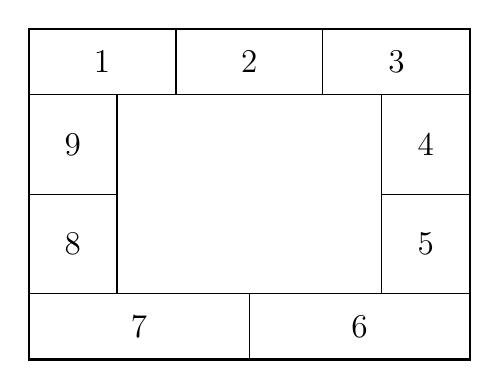
\begin{tikzpicture}[scale=0.7]
  % Draw the corridor as nested rectangles
  \draw[thick] (0,0) rectangle (8,6);
  % Office labels around the perimeter
  % Top: 1, 2, 3
  \draw (0,6) rectangle (2.67,4.8); \node at (1.33, 5.4) {\large 1};
  \draw (2.67,6) rectangle (5.33,4.8); \node at (4, 5.4) {\large 2};
  \draw (5.33,6) rectangle (8,4.8); \node at (6.67, 5.4) {\large 3};
  % Right: 4, 5
  \draw (6.4,4.8) rectangle (8,3); \node at (7.2, 3.9) {\large 4};
  \draw (6.4,3) rectangle (8,1.2); \node at (7.2, 2.1) {\large 5};
  % Bottom: 6, 7
  \draw (4,0) rectangle (8,1.2); \node at (6, 0.6) {\large 6};
  \draw (0,0) rectangle (4,1.2); \node at (2, 0.6) {\large 7};
  % Left: 8, 9
  \draw (0,1.2) rectangle (1.6,3); \node at (0.8, 2.1) {\large 8};
  \draw (0,3) rectangle (1.6,4.8); \node at (0.8, 3.9) {\large 9};
\end{tikzpicture}
\end{center}
Person $P_i$ initially occupies office $i$. The agents' strict preference orderings (listed from most preferred to least preferred) are:
\begin{center}
\begin{tabular}{c|ccccccccc}
  \text{Rank} & $P_1$ & $P_2$ & $P_3$ & $P_4$ & $P_5$ & $P_6$ & $P_7$ & $P_8$ & $P_9$ \\
  \hline
  1 & 7 & 4 & 6 & 7 & 7 & 7 & 9 & 6 & 2 \\
  2 & 6 & 9 & 2 & 1 & 1 & 1 & 3 & 2 & 5 \\
  3 & 9 & 6 & 8 & 5 & 8 & 2 & 6 & 4 & 4 \\
  4 & 4 & 2 & 1 & 8 & 4 & 4 & 2 & 3 & 8 \\
  5 & 8 & 5 & 7 & 9 & 3 & 5 & 5 & 7 & 3 \\
  6 & 5 & 3 & 4 & 3 & 5 & 3 & 4 & 5 & 1 \\
  7 & 1 & 7 & 5 & 2 & 6 & 8 & 8 & 1 & 9 \\
  8 & 2 & 8 & 9 & 6 & 9 & 9 & 7 & 8 & 6 \\
  9 & 3 & 1 & 3 & 4 & 2 & 6 & 1 & 9 & 7 \\
\end{tabular}
\end{center}
\medskip
We apply TTC to the office problem defined above. The logic of each round is as follows:
\begin{itemize}
    \item Every remaining agent \emph{points to} the current owner of their most-preferred available office, forming a directed graph in which each node has out-degree exactly one.
    \item Following the arrows traces directed \textbf{chains}. Because each node has exactly one outgoing edge, every chain must eventually revisit a node---so every chain either \emph{closes into a cycle} or \emph{feeds into} a cycle found by another chain.
    \item \textcolor{MidnightBlue}{\textbf{Cycle members}} trade immediately (each receives the office of the agent they pointed to). \textcolor{gray}{\textbf{Tail agents}} (those whose chains lead into the cycle without closing) are held over for the next round.
\end{itemize}

% ------------------------------------------------------------------
\medskip
\noindent\textbf{Round 1.} All nine agents with offices $\{1,\ldots,9\}$.

\begin{center}
\begin{tikzpicture}[
  >=Stealth,
  cyc/.style  = {circle, draw=MidnightBlue, fill=MidnightBlue!15,
                 thick, minimum size=0.82cm, font=\small\bfseries},
  tail/.style = {circle, draw=gray!70, thick,
                 minimum size=0.82cm, font=\small},
  ce/.style   = {->, MidnightBlue, line width=1.3pt},
  te/.style   = {->, gray!70, dashed, thick}
]
  %% --- Cycle nodes: P7 -> P9 -> P2 -> P4 -> P7 ---
  \node[cyc] (P7) at (2.2, 1.6)  {$P_7$};
  \node[cyc] (P9) at (4.2, 1.6)  {$P_9$};
  \node[cyc] (P2) at (4.2, 0.0)  {$P_2$};
  \node[cyc] (P4) at (2.2, 0.0)  {$P_4$};
  \draw[ce] (P7) -- (P9);
  \draw[ce] (P9) -- (P2);
  \draw[ce] (P2) -- (P4);
  \draw[ce] (P4) -- (P7);

  %% --- Tail nodes ---
  \node[tail] (P6) at (0.4,  0) {$P_6$};
  \node[tail] (P1) at (-1.0, 2.8) {$P_1$};
  \node[tail] (P5) at (-1.0, 1.6) {$P_5$};
  \node[tail] (P3) at (-2.4, 1.5) {$P_3$};
  \node[tail] (P8) at (-2.4, 0) {$P_8$};

  \draw[te] (P1) -- (P7);
  \draw[te] (P5) -- (P7);
  \draw[te] (P6) -- (P7);
  \draw[te] (P3) -- (P6);
  \draw[te] (P8) -- (P6);

  %% --- Labels ---
  \node[MidnightBlue, font=\footnotesize\itshape] at (3.2, 0.8) {cycle};
  \node[gray!80,      font=\footnotesize\itshape] at (-1.5, 3.3) {tails};
\end{tikzpicture}
\end{center}

\noindent\emph{Chains and cycle detection.}
\begin{itemize}
    \item Start from $P_1$: $P_1\!\to\!P_7\!\to\!P_9\!\to\!P_2\!\to\!P_4\!\to\!P_7$ --- the chain revisits $P_7$. \textbf{Cycle found:} $P_7\!\to\!P_9\!\to\!P_2\!\to\!P_4\!\to\!P_7$.
    \item $P_1$ (arriving at $P_7$), as well as $P_5$ (pointing directly to $P_7$), $P_6$ (pointing to $P_7$), $P_3$ and $P_8$ (pointing to $P_6$) are all tails. They do not close any new cycle.
\end{itemize}

\noindent\emph{Cycle trade:}
\[
P_7 \gets \text{office } 9,\quad P_9 \gets \text{office } 2,\quad P_2 \gets \text{office } 4,\quad P_4 \gets \text{office } 7.
\]
Remove $\{P_2, P_4, P_7, P_9\}$ and offices $\{2, 4, 7, 9\}$. Tails $\{P_1, P_3, P_5, P_6, P_8\}$ proceed.

% ------------------------------------------------------------------
\medskip
\noindent\textbf{Round 2.} Remaining agents: $\{P_1, P_3, P_5, P_6, P_8\}$; available offices: $\{1, 3, 5, 6, 8\}$.

\begin{center}
\begin{tikzpicture}[
  >=Stealth,
  cyc/.style  = {circle, draw=MidnightBlue, fill=MidnightBlue!15,
                 thick, minimum size=0.82cm, font=\small\bfseries},
  tail/.style = {circle, draw=gray!70, thick,
                 minimum size=0.82cm, font=\small},
  ce/.style   = {->, MidnightBlue, line width=1.3pt},
  te/.style   = {->, gray!70, dashed, thick}
]
  %% --- Cycle: P1 <-> P6 ---
  \node[cyc] (P1) at (0.0, 0.0) {$P_1$};
  \node[cyc] (P6) at (2.2, 0.0) {$P_6$};
  \draw[ce, bend left=22] (P1) to (P6);
  \draw[ce, bend left=22] (P6) to (P1);

  %% --- Tail nodes ---
  \node[tail] (P5) at (-1.4,  1.2) {$P_5$};
  \node[tail] (P3) at ( 3.6,  1.2) {$P_3$};
  \node[tail] (P8) at ( 3.6, -1.2) {$P_8$};

  \draw[te] (P5) -- (P1);
  \draw[te] (P3) -- (P6);
  \draw[te] (P8) -- (P6);

  \node[MidnightBlue, font=\footnotesize\itshape] at (1.1,  0.7) {cycle};
  \node[gray!80,      font=\footnotesize\itshape] at (-2, 1.65) {tails};
\end{tikzpicture}
\end{center}

\noindent\emph{Chains and cycle detection.}
\begin{itemize}
    \item Start from $P_5$: $P_5\!\to\!P_1\!\to\!P_6\!\to\!P_1$ --- revisits $P_1$. \textbf{Cycle found:} $P_1\!\leftrightarrow\!P_6$.
    \item $P_3$ and $P_8$ both point to $P_6$ (into the cycle), and $P_5$ points to $P_1$ (into the cycle). All three are tails.
\end{itemize}

\noindent\emph{Cycle trade:} $P_1 \gets \text{office } 6,\quad P_6 \gets \text{office } 1.$

\noindent Remove $\{P_1, P_6\}$ and offices $\{1, 6\}$. Tails $\{P_3, P_5, P_8\}$ proceed.

% ------------------------------------------------------------------
\medskip
\noindent\textbf{Round 3.} Remaining: $\{P_3, P_5, P_8\}$; available offices: $\{3, 5, 8\}$.

\begin{center}
\begin{tikzpicture}[
  >=Stealth,
  cyc/.style  = {circle, draw=MidnightBlue, fill=MidnightBlue!15,
                 thick, minimum size=0.82cm, font=\small\bfseries},
  tail/.style = {circle, draw=gray!70, thick,
                 minimum size=0.82cm, font=\small},
  ce/.style   = {->, MidnightBlue, line width=1.3pt},
  te/.style   = {->, gray!70, dashed, thick}
]
  %% --- Cycle: P3 <-> P8 ---
  \node[cyc] (P3) at (0.0, 0.0) {$P_3$};
  \node[cyc] (P8) at (2.2, 0.0) {$P_8$};
  \draw[ce, bend left=22] (P3) to (P8);
  \draw[ce, bend left=22] (P8) to (P3);

  %% --- Tail ---
  \node[tail] (P5) at (1.1, 1.5) {$P_5$};
  \draw[te] (P5) -- (P8);

  \node[MidnightBlue, font=\footnotesize\itshape] at (1.1,  0.65) {cycle};
  \node[gray!80,      font=\footnotesize\itshape] at (1.1,  2.1) {tail};
\end{tikzpicture}
\end{center}

\noindent\emph{Chains and cycle detection.}
\begin{itemize}
    \item $P_3\!\to\!P_8\!\to\!P_3$ --- revisits $P_3$. \textbf{Cycle found:} $P_3\!\leftrightarrow\!P_8$.
    \item $P_5\!\to\!P_8$ feeds into the cycle; $P_5$ is a tail.
\end{itemize}

\noindent\emph{Cycle trade:} $P_3 \gets \text{office } 8,\quad P_8 \gets \text{office } 3.$

\noindent Remove $\{P_3, P_8\}$ and offices $\{3, 8\}$.

% ------------------------------------------------------------------
\medskip
\noindent\textbf{Round 4.} Only $P_5$ remains with office $5$. With a single agent, the ``chain'' is a trivial self-loop: $P_5\!\to\!P_5$. The self-loop is itself a cycle, so $P_5$ keeps office $5$.

% ------------------------------------------------------------------
\medskip
\noindent The final TTC allocation is:
\[
\begin{array}{c|ccccccccc}
  \text{Agent}  & P_1 & P_2 & P_3 & P_4 & P_5 & P_6 & P_7 & P_8 & P_9 \\
  \hline
  \text{Office} &  6  &  4  &  8  &  7  &  5  &  1  &  9  &  3  &  2
\end{array}
\]
}

\rmkb[Cycle Structure in TTC]{
  In each round, the pointing graph is a \textit{functional graph}: every
  node has out-degree exactly one. A fundamental property of functional
  graphs is that each weakly connected component contains \emph{exactly
  one} directed cycle, with all remaining nodes forming tails that feed
  into it. Consequently:
  \begin{itemize}
    \item \textbf{Existence:} At least one cycle is guaranteed to exist
    in every round, since the finite graph must eventually revisit a node
    along any directed path.
    \item \textbf{Multiplicity:} The number of cycles per round equals
    the number of weakly connected components---it may be one or many,
    depending on the preference profile. Uniqueness of cycles \emph{per
    round} does not hold in general.
    \item \textbf{Uniqueness within a chain:} Following the arrows from
    any fixed starting node traces a single directed path, which must
    eventually close into \emph{exactly one} cycle. This per-chain
    uniqueness is what makes TTC well-defined: each agent belongs to at
    most one cycle and receives a unique assignment in the round that
    cycle is identified.
  \end{itemize}
}

\subsection{Properties of TTC}

\subsubsection{TTC Implements the Core}

\thmp{TTC Allocation is in the Core}{
  The allocation produced by the TTC algorithm is in the core of the housing market. Moreover, when preferences are strict, the core contains a unique allocation, and TTC finds it.
}{
  \rmk{
    The intuition is as follows. Agents removed in Round 1 each obtain their overall top choice---no coalition including any of them can make them strictly better off, since they already have their first-best house. Once Round 1 agents are settled, Round 2 agents obtain their best feasible house given Round 1 assignments, and so on. Any blocking coalition would need to offer some agent a house better than what TTC gave them, but that house has already been claimed by someone removed in an earlier round who would never agree to give it up.
  }

  \medskip
  \noindent We proceed by induction on the round of removal. For each
  round $r$, let $C_r$ denote the set of agents removed in round $r$
  (i.e., the union of all cycles identified and executed in that round),
  and let $H_r = \{\mu(i) : i \in C_r\}$ denote the corresponding set
  of houses allocated in round $r$.

  \medskip
  \noindent\textbf{Base case (Round 1).} Every agent removed in Round 1
  belongs to a cycle in which each member points to the owner of their
  globally top-ranked house. Each such agent therefore receives their
  first-best house. No coalition $S$ can block this allocation: to improve
  upon the outcome for any Round-1 agent $i \in S$, the coalition would
  need to reassign $i$'s own top choice to $i$---but $i$ already has it.

  \medskip
  \noindent\textbf{Inductive step.} Suppose that for all rounds $r' < r$,
  the agents removed in rounds $1, \ldots, r'-1$ receive their best
  house within the set of houses held by agents in those same rounds, and
  no coalition can improve upon their assignment using only houses from
  $\bigcup_{r'' \leq r'} H_{r''}$. Consider agents removed in round $r$.
  Each such agent receives their most preferred house among all houses
  still available---i.e., not yet claimed by any agent removed in rounds
  $1, \ldots, r-1$.

  \medskip
  Suppose for contradiction that some blocking coalition $S$ exists.
  Let $i \in S$ be an agent who is made strictly better off under the
  proposed reassignment, and let $h'$ be the house $S$ proposes to give
  $i$, where $h' \succ_i \mu(i)$. Since $\mu(i)$ is already $i$'s best
  available house in round $r$, the house $h'$ must have been removed in
  some earlier round $r' < r$---it belongs to some agent $j \in C_{r'}$
  who exited in round $r'$ with $\mu(j) = h'$. For $S$ to reassign $h'$
  to $i$, it must include $j$. But by the inductive hypothesis, $\mu(j)
  = h'$ is $j$'s best house within $H_{r'}$; giving up $h'$ makes $j$
  strictly worse off, so $j$ would not participate in $S$. Contradiction.

  \medskip
  Hence the TTC allocation is in the core. For uniqueness under strict
  preferences: any core allocation must give Round-1 agents their top
  choice (otherwise the coalition $C_1$ itself is a blocking coalition),
  and by induction any core allocation must coincide with TTC round by
  round. Thus the core is a singleton, and TTC finds it.
}

\corp{TTC is Individually Rational}{
  The allocation produced by TTC is individually rational: every agent
  weakly prefers their assigned house to their own initial endowment.
  That is, $\mu(i) \succsim_i h_i$ for all $i \in \mathcal{P}$.
}{
  This follows immediately from the core property. Suppose for
  contradiction that some agent $i$ strictly prefers their endowment
  to their TTC allocation: $h_i \succ_i \mu(i)$. Then the singleton
  coalition $S = \{i\}$, using the trivial allocation $Q'(i) = h_i$
  (agent $i$ keeps their own house), satisfies $Q'(i) \succ_i \mu(i)$.
  This means $S$ blocks $\mu$, contradicting the fact that $\mu$ is in
  the core. Hence no such $i$ can exist.
}

\subsubsection{TTC is Order Independent}

\thmp{TTC is Order Independent (Strict Preferences)}{
  Suppose all agents have strict preferences over objects. When there
  are multiple cycles in a given round, the TTC outcome does not depend
  on the order in which cycles are identified and removed. That is,
  under strict preferences, the final allocation is unique regardless
  of which cycle is processed first.
}{
  The proof reduces to one key structural observation about functional
  graphs.

  \clmp{}{
    Under strict preferences, in any round of TTC, all cycles in the
    pointing graph are \emph{vertex-disjoint}.
  }{
    Under strict preferences, each agent has a unique top-ranked
    available object, so the pointing graph is a functional graph:
    every node has out-degree exactly one. Suppose for contradiction
    that two distinct cycles $\mathcal{C}_1$ and $\mathcal{C}_2$ share
    a node $v$. Then $v$ would need two distinct outgoing edges---one
    continuing around $\mathcal{C}_1$ and one around $\mathcal{C}_2$---
    contradicting out-degree one. Hence all cycles are vertex-disjoint.
  }

  \medskip
  \noindent Since any two coexisting cycles $\mathcal{C}_1$ and
  $\mathcal{C}_2$ are vertex-disjoint, the agents and houses in
  $\mathcal{C}_1$ are entirely distinct from those in $\mathcal{C}_2$.
  Removing $\mathcal{C}_1$ first therefore does not affect the
  membership or the pointing structure of $\mathcal{C}_2$, and vice
  versa. More precisely:
  \begin{itemize}
    \item The agents in $\mathcal{C}_2$ are still present after
    $\mathcal{C}_1$ is removed, and their preferences over the
    remaining houses are unchanged.
    \item The agents in $\mathcal{C}_2$ still point to the same
    targets they did before (none of their targets were in
    $\mathcal{C}_1$), so $\mathcal{C}_2$ remains a valid cycle in
    the reduced graph.
  \end{itemize}
  By symmetry, removing $\mathcal{C}_2$ first leaves $\mathcal{C}_1$
  intact. In either order, both cycles are eventually removed and
  their members receive exactly the same houses. Since the argument
  applies to every pair of coexisting cycles in every round, the
  final allocation is independent of the order in which cycles are
  processed.
}

\rmkb[Order Dependence Under Weak Preferences]{
  The strictness assumption embedded in our definition of a housing
  market is not merely a technical convenience---it is essential for
  TTC to be well-defined. To see what goes wrong if we relax it,
  suppose we allow agents to be \textit{indifferent} between objects
  (i.e., $\succ_i$ is replaced by a weak order $\succsim_i$). Then
  an agent with multiple top-ranked objects has out-degree greater
  than one in the pointing graph, vertex-disjointness of cycles can
  fail, and different cycle-processing orders may yield different
  allocations.

  \medskip
  \noindent\textbf{Counterexample.} Consider three agents with three
  houses:
  \[
    \text{agent } 1 \text{ owns } A,\quad
    \text{agent } 2 \text{ owns } B,\quad
    \text{agent } 3 \text{ owns } C,
  \]
  with weak preferences $1: B \sim C \succ A$,\quad $2: A \succ B
  \succ C$,\quad $3: A \succ C \succ B$.

  \medskip
  \noindent\textit{Pointing graph.}\quad Agent 1 is indifferent between
  $B$ and $C$ and simultaneously points to both agents 2 and 3. Agents
  2 and 3 each point to agent 1. The resulting graph has out-degree 2
  at node 1, and contains two cycles sharing that node:

  \begin{center}
  \begin{tikzpicture}[>=Stealth, font=\small,
      anode/.style={circle, draw=NavyBlue, fill=NavyBlue!12, thick,
                    minimum size=1.0cm, font=\small\bfseries},
      lbl/.style={font=\footnotesize\itshape, text=gray}
  ]
    %% nodes
    \node[anode] (1) at (0,  0)   {$1$};
    \node[anode] (2) at (-2.2, -1.8) {$2$};
    \node[anode] (3) at ( 2.2, -1.8) {$3$};

    %% labels (owns)
    \node[lbl] at (0,   0.75)  {owns $A$};
    \node[lbl] at (-2.2,-2.55) {owns $B$};
    \node[lbl] at ( 2.2,-2.55) {owns $C$};

    %% agent 1 points to BOTH 2 and 3 (double arrow, BrickRed to signal tie)
    \draw[->, BrickRed, line width=1.2pt, bend right=12]
        (1) to node[midway, left,  font=\scriptsize\color{BrickRed}]
        {$B\sim C$} (2);
    \draw[->, BrickRed, line width=1.2pt, bend left=12]
        (1) to (3);

    %% agent 2 points to 1
    \draw[->, NavyBlue, line width=1.2pt, bend right=12]
        (2) to (1);

    %% agent 3 points to 1
    \draw[->, NavyBlue, line width=1.2pt, bend left=12]
        (3) to (1);

    %% cycle labels
    \node[draw=MidnightBlue, rounded corners, fill=MidnightBlue!6,
          font=\scriptsize, inner sep=3pt]
        at (-1.2, -0.3) {$\mathcal{C}_1$};
    \node[draw=MidnightBlue, rounded corners, fill=MidnightBlue!6,
          font=\scriptsize, inner sep=3pt]
        at ( 1.2, -0.3) {$\mathcal{C}_2$};

    %% shared-node annotation
    \node[BrickRed, font=\scriptsize] at (0, -0.6)
        {\textbf{shared node!}};
  \end{tikzpicture}
  \end{center}

  \noindent The two cycles $\mathcal{C}_1 = (1\!\to\!2\!\to\!1)$ and
  $\mathcal{C}_2 = (1\!\to\!3\!\to\!1)$ are \emph{not} vertex-disjoint.
  Processing them in different orders gives different outcomes:

  \begin{center}
  \begin{tikzpicture}[>=Stealth, font=\small,
      anode/.style={circle, draw, thick, minimum size=0.9cm,
                    font=\small\bfseries},
      hnode/.style={draw, rounded corners=3pt, thick,
                    minimum width=0.75cm, minimum height=0.55cm,
                    font=\small},
      arr/.style={->, thick}
  ]
    %% ---- LEFT PANEL: process C1 first ----
    \begin{scope}[xshift=0cm]
      \node[font=\small\bfseries] at (1.5, 1.8)
          {Process $\mathcal{C}_1$ first};

      % cycle trade
      \node[anode, fill=MidnightBlue!15] (L1) at (0,    0.5) {$1$};
      \node[anode, fill=MidnightBlue!15] (L2) at (2.4,  0.5) {$2$};
      \draw[arr, MidnightBlue] (L1) to[bend left=22]
          node[above, font=\scriptsize]{gets $B$} (L2);
      \draw[arr, MidnightBlue] (L2) to[bend left=22]
          node[below, font=\scriptsize]{gets $A$} (L1);

      % agent 3 keeps C
      \node[anode, fill=gray!15] (L3) at (1.2, -0.9) {$3$};
      \node[font=\scriptsize, gray] at (1.2, -1.65) {keeps $C$};
    \end{scope}

    %% ---- RIGHT PANEL: process C2 first ----
    \begin{scope}[xshift=5.6cm]
      \node[font=\small\bfseries] at (1.5, 1.8)
          {Process $\mathcal{C}_2$ first};

      % cycle trade
      \node[anode, fill=MidnightBlue!15] (R1) at (0,    0.5) {$1$};
      \node[anode, fill=MidnightBlue!15] (R3) at (2.4,  0.5) {$3$};
      \draw[arr, MidnightBlue] (R1) to[bend left=22]
          node[above, font=\scriptsize]{gets $C$} (R3);
      \draw[arr, MidnightBlue] (R3) to[bend left=22]
          node[below, font=\scriptsize]{gets $A$} (R1);

      % agent 2 keeps B
      \node[anode, fill=gray!15] (R2) at (1.2, -0.9) {$2$};
      \node[font=\scriptsize, gray] at (1.2, -1.65) {keeps $B$};
    \end{scope}

    %% divider
    \draw[dashed, gray] (4, -2.0) -- (4, 2.1);

    %% outcome tables
    \node[font=\scriptsize] at (1.5, -2.4)
        {$1\!\gets\!B,\quad 2\!\gets\!A,\quad 3\!\gets\!C$};
    \node[font=\scriptsize] at (7.1, -2.4)
        {$1\!\gets\!C,\quad 2\!\gets\!B,\quad 3\!\gets\!A$};
  \end{tikzpicture}
  \end{center}

  \noindent The two orders produce distinct allocations, confirming
  that TTC is not well-defined under weak preferences without an
  additional tie-breaking rule.

  \medskip
  The standard remedy is to impose an exogenous \textbf{tie-breaking
  rule} (e.g., a lottery over objects) before running TTC, converting
  weak preferences into strict ones. This restores out-degree one,
  vertex-disjoint cycles, and a well-defined outcome. However, the
  final allocation then depends on the tie-breaking rule chosen, so
  TTC under weak preferences is best understood as a \textit{family}
  of mechanisms indexed by tie-breaking rules, rather than a single
  deterministic procedure.
}

\subsubsection{TTC is Strategy-Proof}

\thmp{TTC is Individual Strategy-Proof}{
  Under the TTC mechanism, truthful reporting of preferences is a
  dominant strategy for every agent. That is, regardless of what other
  agents report, no agent can obtain a strictly better outcome by
  misreporting their preferences.
}{
  Fix any agent $i$ and any reports $P_{-i}$ by all other agents. Let
  $\mu$ denote the TTC outcome under truthful reporting, with $\mu(i) =
  o^*$, and let $r$ be the round in which $i$ exits under truthful TTC.
  We show that no misreport $P_i'$ yields $i$ a strictly better object.

  \medskip
  \noindent\textbf{Key observation.} An agent's report determines only
  \emph{whom they point to}; it does not affect whom others point to.
  Since all $j \neq i$ report truthfully, the pointing behavior of every
  $j \neq i$ depends only on $j$'s own preferences and the current
  available set---both of which are unaffected by $i$'s report.

  \medskip
  We present two proofs, each illuminating a different aspect of the
  mechanism.

  \medskip
  \noindent\textbf{Proof 1 (by contradiction on the object obtained).}
  Suppose $i$ misreports and obtains $o' \succ_i o^*$. We derive a
  contradiction in two cases.

  \begin{itemize}
    \item \textbf{Case 1: $o'$ was taken in round $r' < r$ under
    truth-telling.} For $i$ to obtain $o'$, $i$ must be part of the
    cycle containing $o'$ in round $r'$ under the misreport. This
    requires some agent $j \neq i$ to point to $i$ in round $r'$,
    closing the cycle through $i$. But $j$'s pointing depends only on
    $j$'s preferences and the available set at round $r'$. As long as
    $i$ is still present at round $r'$, the agents and objects removed
    in rounds $1, \ldots, r'-1$ are exactly those from cycles not
    involving $i$---the same as under truth-telling (since those cycles
    form independently of $i$'s report). Hence the available set at
    round $r'$ is identical under both runs, and so is $j$'s pointing.
    Since no $j$ points to $i$ in round $r'$ under truth-telling (no
    cycle involving $i$ forms before round $r$), no $j$ does so under
    misreport either. The cycle closes without $i$. Contradiction.

    \item \textbf{Case 2: $o'$ is available in round $r$ under
    truth-telling.} Then $o' \in A_r$, the available set when $i$'s
    truthful cycle forms. But under truth-telling $i$ points to the
    owner of their top choice in $A_r$, which would be $o'$ if $o'
    \succ_i o^*$---contradicting $\mu(i) = o^*$.
  \end{itemize}

  \medskip
  \noindent\textbf{Proof 2 (by analyzing the exit round).}
  Suppose $i$ misreports and exits in round $r' \neq r$. We show
  neither case improves $i$'s outcome.

  \begin{itemize}
    \item \textbf{Case 1: $r' > r$ (i exits later).} In TTC, each
    agent exits in the round their cycle forms, receiving their most
    preferred object among those still available \emph{at that round}.
    By construction, $A_{r'} \subseteq A_r$: the longer $i$ stays, the
    more objects get claimed by earlier cycles. Hence $i$'s best
    available object weakly worsens as the round increases, and exiting
    later cannot improve $i$'s outcome.

    \item \textbf{Case 2: $r' < r$ (i exits earlier).} For $i$ to exit
    in round $r' < r$, $i$ must join a cycle in that round. This
    requires some $j \neq i$ to point toward $i$ (to close the cycle
    through $i$). Under truth-telling, $j$ points to $i$ in round $r'$
    if and only if $h_i$ is $j$'s top available object at round $r'$.
    Since the available set at round $r'$ is the same under both runs
    (cycles before round $r'$ do not involve $i$ and form identically),
    $j$ already points to $i$ in round $r'$ under truth-telling. But
    then $j$ never exits before round $r'$, so $j$ is still present in
    round $r$ under truth-telling. This means $h_j \in A_r$, the
    available set when $i$ exits truthfully. Since $\mu(i) = o^*$ is
    $i$'s top choice from $A_r$ and $h_j \in A_r$, we have $o^*
    \succsim_i h_j$. Joining $j$'s cycle early to obtain $h_j$ cannot
    improve upon $o^*$.
  \end{itemize}

  In all cases, no misreport yields $i$ a strictly better object than
  $o^*$. Since $i$ and $P_{-i}$ were arbitrary, truth-telling is a
  dominant strategy for every agent.
}

The two proofs above capture complementary intuitions about why
  manipulation fails in TTC.
\begin{itemize}
  \item \textbf{Proof 1} asks: \textit{can $i$ obtain a specific better
  object $o'$?} It shows the answer is no by ruling out each possible
  location of $o'$: either $o'$ was already taken (and $i$ cannot
  intercept its cycle, since no one points back to $i$), or $o'$ was
  available all along (and $i$ would have gotten it honestly).
  \item \textbf{Proof 2} asks: \textit{can $i$ benefit by changing which
  round it exits?} It shows the answer is no in both directions.
  Exiting later only shrinks the available set. Exiting earlier forces
  $i$ to join a chain that was already pointing toward $i$ under
  truth-telling---meaning the object at the end of that chain was
  already in $i$'s truthful available set $A_r$, and therefore no
  better than $o^*$.
\end{itemize}

  At the deepest level, both proofs rest on the same asymmetry:
  \textit{$i$ controls only whom it points to, not who points back.}
  The objects reachable by $i$ are ultimately determined by who is
  willing to trade with $i$---and that depends on others' preferences,
  which no misreport can change.

A natural follow-up question is whether TTC is also
  \textit{group strategy-proof}: can a coalition of agents coordinate
  their misreports to make every member of the coalition strictly better
  off? The answer is \textbf{NO}---TTC is group strategy-proof. No
  coalition can jointly misreport preferences and make all coalition
  members strictly better off.
  This is a stronger result that follows from the fact that TTC
  implements the unique strict core allocation, combined with the
  structure of the trading cycle procedure.

\thmp{TTC is Strictly Group Strategy-Proof}{
  TTC is group strategy-proof: there is no coalition $S \subseteq \P$
  and no coordinated misreport $P_S'$ such that every member of $S$
  obtains a strictly better object than under truthful reporting.
}{
  \rmk{
    The proof has two parts that mirror---and extend---the individual
    strategy-proofness argument. Individual SP shows that no single
    agent can infiltrate a better cycle, because they cannot control
    who points back to them. Group SP faces a richer challenge: even
    if coalition members coordinate their pointing, they still cannot
    control the pointing of agents outside $S$, and---crucially---the
    core uniqueness of TTC prevents them from profitably rearranging
    objects among themselves either.
  }

  \medskip
  Suppose for contradiction that $S$ misreports $P_S'$ and obtains
  allocation $\mu'$ with $\mu'(i) \succ_i \mu(i)$ for all $i \in S$,
  where $\mu$ is the truthful TTC outcome. Partition $S$'s gains by
  the origin of the improved objects: outside $S$, and inside $S$ (redistribution).

  \clmp{}{
No $S$-member can gain an object initially
  owned by an agent outside $S$.
  }{
    Suppose $i \in S$ gains object $o' = \mu'(i) \succ_i \mu(i)$, where
  $o'$ is initially owned by some $j \notin S$. Fix the reports of all
  other agents at $(P_{S \setminus \{i\}}',\, P_{-S})$ and apply the
  individual strategy-proofness argument to $i$ alone. Regardless of
  what others report, $i$ cannot benefit from misreporting; in
  particular, the same two-case argument applies verbatim:

  \begin{itemize}
    \item If $o'$ was removed in an earlier round under this fixed
    profile, $j \notin S$ reports truthfully, so $j$'s pointing
    behavior depends only on $j$'s own preferences and the available
    set---neither of which $i$'s report can affect. No agent in the
    cycle containing $o'$ points back to $i$, so $i$ cannot join that
    cycle regardless of $i$'s misreport. Contradiction.

    \item If $o'$ is still available in $i$'s exit round, then $o'
    \succ_i \mu(i)$ implies $i$ would have pointed to $j$ (owner of
    $o'$) under truthful reporting and obtained $o'$ honestly---
    contradicting $\mu(i) \neq o'$.
  \end{itemize}

  Hence every $i \in S$ can only gain objects initially endowed to
  other $S$-members. That is, $\{\mu'(i) : i \in S\} \subseteq
  \{h_i : i \in S\}$.
  }

  \clmp{}{
$S$ cannot profitably redistribute its own
  endowments.
  }{
By the previous claim, the objects received by $S$-members under $\mu'$ are
  drawn entirely from $\{h_i : i \in S\}$. Define an allocation $\nu$
  for $S$ by $\nu(i) = \mu'(i)$ for all $i \in S$. Then $\nu$ is a
  redistribution of $\{h_i : i \in S\}$ among $S$ such that $\nu(i)
  \succ_i \mu(i)$ for all $i \in S$. This means $S$ constitutes a
  \emph{blocking coalition} for $\mu$ under true preferences,
  contradicting the fact that $\mu$ is in the strict core.
  }

  Both parts yield contradictions, so no coalition $S$ can jointly
  misreport to make all its members strictly better off.
}

\thmp{TTC is Weakly Group Strategy-Proof}{
  The TTC mechanism is weakly group strategy-proof: there is no
  coalition $S \subseteq \P$ and joint misreport $P_S'$ such that
  the resulting outcome $\mu'$ satisfies
  \[
    \mu'(i) \succsim_i \mu(i) \;\text{ for all } i \in S,
    \quad\text{with}\quad
    \mu'(i^*) \succ_{i^*} \mu(i^*) \;\text{ for some } i^* \in S.
  \]
}{
  Suppose for contradiction that such $S$ and $P_S'$ exist. Since
  preferences are strict, every $i \in S$ either keeps exactly the
  same object ($\mu'(i) = \mu(i)$) or gets a strictly better one.
  Partition $S$ accordingly:
  \[
    S^+ = \{i \in S : \mu'(i) \succ_i \mu(i)\} \neq \emptyset,
    \qquad
    S^0 = \{i \in S : \mu'(i) = \mu(i)\}.
  \]

  Run TTC under the misreport profile $(P_S', P_{-S})$. Among all
  $S^+$-members, let $r^*$ be the earliest round in which any
  $S^+$-member exits, and let $i^{**} \in S^+$ be such a member.
  Let $\mathcal{C}$ be the TTC cycle that $i^{**}$ belongs to in
  round $r^*$.

  In cycle $\mathcal{C}$, agents trade their initial endowments
  cyclically: writing $\mathcal{C} = (a_1 \to a_2 \to \cdots
  \to a_k \to a_1)$, each $a_l$ gets $h_{a_{l+1}}$ (indices mod
  $k$). In particular, $\mu'(a_l) = h_{a_{l+1}}$ for each $l$.

  \medskip
  \noindent\textbf{Case 1: $\mathcal{C} \subseteq S$.}

  All members of $\mathcal{C}$ belong to $S$, so by the weak
  improvement assumption,
  \[
    \mu'(a_l) = h_{a_{l+1}} \succsim_{a_l} \mu(a_l)
    \quad\text{for all } a_l \in \mathcal{C},
  \]
  with $h_{a_{l^*+1}} \succ_{i^{**}} \mu(i^{**})$ for $i^{**} \in
  \mathcal{C}$. The coalition $\mathcal{C}$ can execute exactly this
  trade under their \emph{true} preferences: each $a_l$ contributes
  endowment $h_{a_l}$ and receives $h_{a_{l+1}}$, a redistribution
  of $\{h_{a_l} : a_l \in \mathcal{C}\}$. Every member weakly
  benefits, and $i^{**}$ strictly benefits. This means $\mathcal{C}$
  is a blocking coalition for $\mu$ under true preferences,
  contradicting the fact that $\mu$ is in the strict core.

  \medskip
  \noindent\textbf{Case 2: $\mathcal{C} \not\subseteq S$.}

  $\mathcal{C}$ contains $i^{**} \in S^+$ and at least one agent
  $j_0 \notin S$. We consider two sub-cases based on whether the
  non-$S$ members of $\mathcal{C}$ are harmed by the trade.

  \medskip
  \noindent\textbf{Sub-case 2a:} $\mu'(j) = h_{n(j)} \succsim_j
  \mu(j)$ for every $j \in \mathcal{C} \setminus S$.

  Then every agent in $\mathcal{C}$ weakly benefits from the cycle
  trade (under true preferences), and $i^{**}$ strictly benefits.
  Again, $\mathcal{C}$ is a blocking coalition for $\mu$,
  contradicting the strict core.

  \medskip
  \noindent\textbf{Sub-case 2b:} Some $j_0 \in \mathcal{C} \setminus
  S$ is strictly harmed: $\mu'(j_0) \prec_{j_0} \mu(j_0)$.

  Let $\mu(j_0) = h_l$ (the object $j_0$ receives under truthful
  TTC, which is $l$'s endowment). Since $j_0$ reports truthfully
  in the misreport run and always picks their top available object,
  the fact that $j_0$ gets $\mu'(j_0) \prec_{j_0} h_l$ at round
  $r^*$ means $h_l$ is \emph{not available} at the start of round
  $r^*$ in the misreport run. So $h_l$ was taken in some round
  $r' < r^*$ by some agent $m \neq j_0$.

  We now derive a contradiction by tracing who took $h_l$:

  \begin{itemize}
    \item $m \notin S^+$: by choice of $r^*$, no $S^+$-member exits
    before round $r^*$. So $m \notin S^+$.

    \item $m \notin S^0$: if $m \in S^0$, then $\mu'(m) = \mu(m)$.
    In round $r'$, $m$ exits and gets $h_l$, so $\mu'(m) = h_l$.
    But then $\mu(m) = h_l = \mu(j_0)$, implying $m = j_0$ (since
    $\mu$ is a bijection). This contradicts $m \in S^0 \subseteq S$
    and $j_0 \notin S$.

    \item Therefore $m \notin S$, and $m$ reports truthfully. In the
    truthful run, $m$'s exit cycle forms at round $r_m$ (the round
    $m$ exits under truth-telling). Under truthful TTC, $m$ gets
    $\mu(m) \neq h_l$ (since $\mu^{-1}(h_l) = j_0 \neq m$ and
    $\mu$ is a bijection). So $m$ is \emph{not} in the cycle
    containing $l$ in the truthful run: under truthful TTC, $m$
    does not point to $l$ at the round where $h_l$ changes hands.
  \end{itemize}

  So in the misreport run, the truthful agent $m \notin S$ ends up
  in a different cycle than in the truthful run, specifically one
  that includes $l$ and yields $h_l$ to $m$. Since $m$ always
  reports truthfully, $m$'s pointing changes only if the available
  set at $m$'s exit round changes. This change in the available set
  must itself be caused by some $S$-member's misreport altering an
  earlier cycle. Tracing this chain: let $\mathcal{C}'$ be the TTC
  cycle in round $r'$ that contains $m$ (and $l$) in the misreport
  run. By the same case analysis applied to $\mathcal{C}'$:

  \begin{itemize}
    \item If $\mathcal{C}' \subseteq S$: a sub-coalition of $S$ is
    trading endowments in $\mathcal{C}'$. Since $m \notin S$ is in
    $\mathcal{C}'$, this is impossible.

    \item If $\mathcal{C}' \not\subseteq S$: $\mathcal{C}'$ contains
    some $S$-member. If all agents in $\mathcal{C}'$ weakly benefit
    (sub-case 2a for $\mathcal{C}'$), then $\mathcal{C}'$ is a
    blocking coalition---contradiction. If some agent in $\mathcal{C}'
    \setminus S$ is strictly harmed, the same tracing argument
    applies recursively to a strictly earlier round.
  \end{itemize}

  Since the rounds are finite and strictly decreasing at each
  recursive step, this process must terminate. The terminal case
  is either sub-case 2a (blocking coalition, contradiction with
  core) or Case~1 (coalition entirely within $S$, contradiction
  with core). Either way, we reach a contradiction.

  \medskip
  Since all cases yield contradictions, no coalition $S$ can
  achieve a weak Pareto improvement via coordinated misreporting.
  TTC is weakly group strategy-proof. 
}

\rmkb[Why Weak GSP Is Harder Than Strong GSP]{
  The additional difficulty in the weak GSP proof relative to strong
  GSP comes entirely from $S^0$-members. In strong GSP, every
  coalition member is assumed strictly better off, so individual
  strategy-proofness can be applied to each member to show they
  can only receive objects from within $S$ (Claim~1 of the strong
  GSP proof). This argument fails for $S^0$-members: they are
  indifferent between their truthful and misreport outcomes, so
  ISP provides no constraint on where their object originates.

  \medskip
  $S^0$-members may misreport not to benefit themselves, but to
  act as ``facilitators''---adjusting the cycle structure in early
  rounds to create a path that allows $S^+$-members to enter
  better cycles. Sub-case 2b captures exactly this scenario and
  requires the recursive tracing argument above: each step of the
  chain that $S^0$-members create must eventually close into a
  cycle, and that cycle is forced to be a blocking coalition for
  $\mu$ under true preferences---which is impossible since $\mu$
  is the unique strict core.
}

\section{The Assignment Problem: Allocation without Endowments}

The housing market model rests critically on the assumption that each
agent holds an initial endowment: this is what gives IR its bite, and
what makes the core a meaningful solution concept. Once we drop this
assumption---handing all objects to a central planner and asking how to
distribute them from scratch---both IR and the core lose their reference
point. We enter the \textit{assignment problem}, where no agent has a
prior claim to any object and the relevant normative goals reduce to
\textit{Pareto efficiency} and \textit{strategy-proofness}.

\subsection{Serial Dictatorship (SD)}

The serial dictatorship (SD) mechanism addresses this setting directly.
Agents are given a predetermined priority ordering and pick their
favorite available object in turn. Compared to TTC, SD trades the
structural richness of cycle-based trading for sheer simplicity: there
are no endowments to track, no cycles to identify, and no core to
verify---just a queue and a sequence of greedy choices.

\state{Serial Dictatorship}{
  Fix an ordering $\sigma = (\sigma(1), \sigma(2), \ldots, \sigma(n))$ of the agents. The mechanism proceeds as follows:
  \begin{enumerate}
    \item Agent $\sigma(1)$ (the ``dictator'') picks their most preferred house from $H$.
    \item Agent $\sigma(2)$ picks their most preferred house from the remaining houses.
    \item Continue until all agents are assigned.
  \end{enumerate}
}

\ex[Serial Dictatorship on the Office Problem]{
  We run SD on the office problem with the natural ordering $\sigma =
  (P_1, P_2, \ldots, P_9)$. At each step, the active agent scans their
  preference list top-to-bottom and picks the highest-ranked office that
  is still available. Taken offices are shown in gray.

  \medskip
  \begin{center}
  \renewcommand{\arraystretch}{1.3}
  \begin{tabular}{c|l|c|c}
    \textbf{Step} & \textbf{Available offices} & \textbf{Agent picks} & \textbf{Gets} \\
    \hline
    1 & $\{1,2,3,4,5,6,7,8,9\}$
      & $P_1$: top choice is $7$ $\checkmark$
      & $7$ \\
    2 & $\{1,2,3,4,5,6,8,9\}$
      & $P_2$: top choice is $4$ $\checkmark$
      & $4$ \\
    3 & $\{1,2,3,5,6,8,9\}$
      & $P_3$: top choice is $6$ $\checkmark$
      & $6$ \\
    4 & $\{1,2,3,5,8,9\}$
      & $P_4$: $7$ taken; next available: $1$ $\checkmark$
      & $1$ \\
    5 & $\{2,3,5,8,9\}$
      & $P_5$: $7,1$ taken; next available: $8$ $\checkmark$
      & $8$ \\
    6 & $\{2,3,5,9\}$
      & $P_6$: $7,1$ taken; next available: $2$ $\checkmark$
      & $2$ \\
    7 & $\{3,5,9\}$
      & $P_7$: top choice is $9$ $\checkmark$
      & $9$ \\
    8 & $\{3,5\}$
      & $P_8$: $6,2,4$ taken; next available: $3$ $\checkmark$
      & $3$ \\
    9 & $\{5\}$
      & $P_9$: $2$ taken; next available: $5$ $\checkmark$
      & $5$ \\
  \end{tabular}
  \end{center}

  \medskip
  \noindent The SD allocation under ordering $\sigma = (P_1, \ldots, P_9)$
  is:
  \[
    \begin{array}{c|ccccccccc}
      \text{Agent}  & P_1 & P_2 & P_3 & P_4 & P_5 & P_6 & P_7 & P_8 & P_9 \\
      \hline
      \text{Office} &  7  &  4  &  6  &  1  &  8  &  2  &  9  &  3  &  5
    \end{array}
  \]

  \noindent Compare this with the TTC allocation on the same problem:
  \[
    \begin{array}{c|ccccccccc}
      \text{Agent}  & P_1 & P_2 & P_3 & P_4 & P_5 & P_6 & P_7 & P_8 & P_9 \\
      \hline
      \text{Office} &  6  &  4  &  8  &  7  &  5  &  1  &  9  &  3  &  2
    \end{array}
  \]
  Several agents differ: $P_1$ gets office $7$ under SD (their top choice)
  versus $6$ under TTC; $P_4$ gets $1$ under SD versus $7$ under TTC.
  This illustrates a key tradeoff: the agent who goes first under SD
  always receives their top choice, but later agents may fare worse than
  under TTC, where the cycle structure can give non-first agents access
  to offices they could not reach by waiting their turn.
}

\subsection{Properties of SD}

\thmp{Serial Dictatorship is Pareto Efficient}{
  The allocation produced by SD is Pareto efficient: there is no other
  allocation that makes every agent weakly better off and some agent
  strictly better off.
}{
  \rmk{
    The argument is essentially one of optimality at the margin. Consider
  the first agent $i$ who would need to be reassigned to achieve the
  supposed Pareto improvement. Agent $i$ already holds their top choice
  among everything not taken by higher-priority agents---there is simply
  nothing better left for them. Any Pareto improvement for $i$ is
  therefore impossible, and the supposed dominating allocation cannot
  exist.
  }
  
  \medskip
  Suppose for contradiction that some allocation $\mu'$ Pareto dominates
  the SD allocation $\mu$. Let $i = \sigma(k)$ be the \emph{first} agent
  in the priority ordering such that $\mu'(i) \neq \mu(i)$. Since $\mu'$
  Pareto dominates $\mu$, we have $\mu'(i) \succ_i \mu(i)$.

  \medskip
  But $\mu(i)$ is $i$'s most preferred object among all objects available
  when it was $i$'s turn---that is, among all objects not already taken
  by $\sigma(1), \ldots, \sigma(k-1)$. Since $i$ is the first agent to
  differ between $\mu$ and $\mu'$, every agent $\sigma(1), \ldots,
  \sigma(k-1)$ receives the same object under both $\mu$ and $\mu'$.
  Therefore the set of objects available to $i$ at step $k$ is identical
  under both allocations, and $\mu(i)$ is $i$'s top choice from that set.
  The existence of $\mu'(i) \succ_i \mu(i)$ with $\mu'(i)$ in the same
  available set is a contradiction.

  \medskip
  \rmk{
    Notice that this argument does \textbf{not} require every agent to get
  their globally top-ranked object. It only requires that each agent gets
  their top choice \textbf{given the residual supply}, which is precisely
  what the greedy sequential structure of SD guarantees.
  }
}

\thmp{Serial Dictatorship is Strategy-Proof}{
  Under SD, truthful reporting of preferences is a dominant strategy for
  every agent. No agent can obtain a strictly better object by
  misreporting their preferences, regardless of what other agents report.
}{
  \rmk{
    In SD, your report only
  affects \emph{what you pick}---it has no effect whatsoever on what is
  available to you, since the available set is determined entirely by
  agents ahead of you in the queue. You always face the same menu $A_k$,
  and truth-telling simply ensures you pick your genuine favorite from
  it. Lying can only cause you to pick something you like less.
  }
  
  Fix any agent $i = \sigma(k)$ and any reports by all other agents.
  Suppose $i$ misreports, yielding object $o'$ under the misreport,
  compared to $o^* = \mu(i)$ under truthful reporting. We show $o'
  \not\succ_i o^*$.

  \medskip
  The key observation is that, the set of objects available to $i$
  at step $k$ is determined entirely by the choices of $\sigma(1), \ldots,
  \sigma(k-1)$, each of whom picks their own top available object
  according to their own report. Since $i = \sigma(k)$ has no influence
  over any earlier agent's report or choice, the available set $A_k$ at
  step $k$ is \textbf{identical} whether $i$ reports truthfully or not.

  \medskip
  Under truthful reporting, $i$ picks $o^* = \mu(i)$, their most preferred
  object in $A_k$ (the available set at step $k$). Under misreport, $i$ picks according to a false
  preference list, and receives some $o' \in A_k$. Since $o^*$ is $i$'s
  true top choice from $A_k$ and $o' \in A_k$, we have $o^* \succsim_i
  o'$. In particular, $o' \not\succ_i o^*$. Since the reports of other
  agents and the choice of $i = \sigma(k)$ were arbitrary, truth-telling
  is a dominant strategy.
}

\subsection{Equivalence of Random SD and TTC with Random Endowments}

The separation between the housing market (with endowments, TTC) and
the assignment problem (without endowments, SD) may seem sharp. Yet
there is a striking bridge between the two frameworks: once we
introduce randomness into either model in the natural way, the two
mechanisms become outcome-equivalent. This result, due to
Abdulkadiro\u{g}lu and S\"{o}nmez (1998), reveals that the
endowment structure and the priority structure are, at a deeper level,
two sides of the same coin.

\medskip
The key observation is that both frameworks have one remaining degree
of freedom that the model leaves unspecified:
\begin{itemize}
  \item In the \textit{assignment problem}, objects have no owner, so
  the mechanism designer must choose a \textbf{priority ordering} over
  agents. If this choice seems arbitrary, a natural response is to
  randomize: draw a uniformly random ordering.
  \item In the \textit{housing market}, agents must have initial
  endowments, but if no agent has a natural prior claim to any
  particular object, a natural response is again to randomize: draw a
  uniformly random endowment assignment, then run TTC.
\end{itemize}
Randomizing the one free parameter in each model yields two
randomized mechanisms. The theorem below says they are the same
mechanism.

\defn{Randomized Mechanisms}{
  \begin{itemize}
    \item \textbf{Random Serial Dictatorship (RSD):} Draw a uniformly
    random ordering $\sigma$ of agents (each of the $n!$ orderings
    equally likely), then run SD under $\sigma$.
    \item \textbf{Core from Random Endowments (CFRE):} Draw a
    uniformly random assignment of objects to agents as initial
    endowments (each of the $n!$ bijections equally likely), then run
    TTC to find the core allocation.
  \end{itemize}
}

\thmp{RSD $=$ CFRE}{
  RSD and CFRE induce the \emph{same} probability distribution over
  allocations: for every deterministic allocation $\mu$,
  \[
    \text{Pr}_{\sigma}\!\bigl[\mu^{\mathrm{SD}}_\sigma = \mu\bigr]
    \;=\;
    \text{Pr}_{e}\!\bigl[\mu^{\mathrm{TTC}}_e = \mu\bigr],
  \]
  where $\sigma$ is a uniformly random priority ordering and $e$ is a
   uniformly random endowment assignment.
}{
\lemp{Within-Cycle Commutativity}{
  Fix any endowment $e$ and let $\mu = \mu^{\mathrm{TTC}}_e$, with TTC
  producing cycles $C_1, C_2, \ldots, C_m$ in successive rounds. Let
  $\Sigma(\mu, e)$ denote the set of all priority orderings that:
  \begin{enumerate}
    \item place all agents in $C_k$ before all agents in $C_{k+1}$
    (for each $k$), and
    \item within each $C_k$, use any permutation of its members.
  \end{enumerate}
  Then SD under every $\sigma \in \Sigma(\mu, e)$ produces $\mu$.
}{
  We establish one fact about the TTC cycle structure.

  \fact{Within-Cycle Self-Preference}{
    For any cycle $C_k$ and any two distinct members $a, b \in C_k$:
  $\mu(a) \succ_a \mu(b)$.
  }
  Take any $\sigma \in \Sigma(\mu, e)$ and any agent $a \in C_k$.
  When $a$'s turn comes in SD, the available objects are a subset
  of those available in TTC round $k$, for the following reason:
  the objects removed before round $k$ in TTC are exactly
  $\bigcup_{l < k}\{\mu(x) : x \in C_l\}$, and by definition of
  $\Sigma(\mu,e)$, all agents in $C_1, \ldots, C_{k-1}$ pick before
  $a$. By the Fact above and induction, each such agent picks their
  own $\mu$-assignment, so the objects removed before $a$'s turn in
  SD are exactly $\bigcup_{l<k}\{\mu(x):x\in C_l\}$ plus the
  $\mu$-assignments of those $C_k$-members who pick before $a$.

  \medskip
  We verify that $\mu(a)$ is $a$'s top available object when $a$
  picks:
  \begin{itemize}
    \item \textbf{Objects from earlier cycles are unavailable.}
    All $\mu(i)$ for $i \in C_l$, $l < k$ have been claimed. In
    TTC, $\mu(a)$ is $a$'s top choice among all objects available
    in round $k$---this already accounts for the absence of earlier
    objects. So no unavailable object is preferred over $\mu(a)$.
    \item \textbf{$\mu(a)$ has not been taken by earlier $C_k$
    members.} By the Fact, every other $b \in C_k$ prefers $\mu(b)$
    over $\mu(a)$, so no earlier $C_k$-member claims $\mu(a)$.
    \item \textbf{Objects from later cycles are weakly worse.}
    All objects $\mu(x)$ for $x \in C_l$, $l > k$ were available
    in TTC round $k$, and $a$ chose $\mu(a)$ over all of them.
  \end{itemize}
  Therefore $a$ claims $\mu(a)$ in SD. Since $a$ was arbitrary,
  SD under $\sigma$ produces $\mu$.
}

  It remains to show that the randomization in CFRE and RSD induce
  the same distribution. We do this by mapping both the valid orderings 
  $\sigma$ and the valid endowments $e$ to a canonical block partition 
  uniquely defined by $\mu$ and the agents' preferences.

  Fix an allocation $\mu$. Define an ordered partition $\mathcal{B} = (B_1, B_2, \ldots, B_m)$ 
  of the agents recursively as follows: Let $B_1$ be the minimal nonempty 
  set of agents whose top choices among all objects are exactly $\mu(B_1)$. 
  Let $B_2$ be the minimal nonempty set of agents whose top choices among 
  the remaining objects $N \setminus \mu(B_1)$ are exactly $\mu(B_2)$, and so on. 
  Notice that $\mathcal{B}$ is uniquely determined independent of $\sigma$ or $e$.

  \medskip
  \noindent \textbf{Counting Orderings for RSD:} \\
  An ordering $\sigma$ yields $\mu$ under SD if and only if it respects this 
  dependency structure. Specifically, agents in $B_k$ must appear after all 
  agents in $B_1, \ldots, B_{k-1}$ to ensure their preferred objects in those 
  blocks are already taken. Because $B_k$ is defined as the minimal closed set 
  under top available choices, the agents within $B_k$ can be processed in 
  \emph{any} internal order without disrupting the assignment $\mu$. 
  Thus, the total number of orderings yielding $\mu$ is exactly the number of 
  ways to permute agents within each block:
  \[
    \bigl|\{ \sigma : \mu^{\mathrm{SD}}_\sigma = \mu \}\bigr| = \prod_{k=1}^m |B_k|!
  \]

  \medskip
  \noindent \textbf{Counting Endowments for CFRE:} \\
  An endowment $e$ yields $\mu$ under TTC if and only if for every block $k$, 
  $e$ endows the objects $\mu(B_k)$ strictly to the agents in $B_k$ 
  (i.e., $e(B_k) = \mu(B_k)$). To see why, consider the TTC pointer function 
  $p(i) = e^{-1}(\mu(i))$. If $e(B_k) = \mu(B_k)$, then $p$ forms a bijection 
  from $B_k$ to itself. Consequently, $p$ perfectly decomposes into a set of 
  disjoint cycles covering all of $B_k$. Since their top available choices 
  are in $\mu(B_k)$, every agent $i \in B_k$ participates in a cycle and 
  receives exactly $\mu(i)$.
  
  The number of such valid endowments is simply the number of possible bijections 
  from $B_k$ to $\mu(B_k)$ for each block $k$. Therefore:
  \[
    \bigl|\{ e : \mu^{\mathrm{TTC}}_e = \mu \}\bigr| = \prod_{k=1}^m |B_k|!
  \]

  \medskip
  Since there are exactly $n!$ total orderings and $n!$ total endowments, 
  and the sizes of the pre-images yielding $\mu$ are strictly equal, we conclude:
  \[
    \text{Pr}_{\sigma}\!\bigl[\mu^{\mathrm{SD}}_\sigma = \mu\bigr] 
    = \frac{\prod_{k=1}^m |B_k|!}{n!} 
    = \text{Pr}_{e}\!\bigl[\mu^{\mathrm{TTC}}_e = \mu\bigr]
  \]
  This holds for any deterministic allocation $\mu$, completing the proof.
}

\rmkb[Proof Intuition]{
  The bijection has a clean interpretation. In SD, the priority
  ordering determines who gets served first. In TTC, the endowment
  determines who holds what. The bijection $\sigma \mapsto e(\sigma)$
  encodes the SD priority order \emph{into} the endowment structure by
  a cyclic shift: agent $\sigma_k$ is endowed with the object that
  $\sigma_{k-1}$ ends up with under SD. This creates a pointing chain
  in TTC that exactly mirrors the SD queue---agent $\sigma_k$ points
  to $\sigma_{k+1}$ because $\sigma_{k+1}$ holds what $\sigma_k$
  ultimately wants. The TTC cycles that form then execute the same
  trades as the SD steps, in the same order.

  \medskip
  At a higher level, both mechanisms are doing the same thing:
  translating an underlying permutation (of agents, or of objects) into
  an allocation by a greedy sequential procedure. Randomizing the
  permutation uniformly in either case produces the same lottery,
  because the two ``greedy procedures'' are isomorphic via the cyclic
  shift bijection.
}

The equivalence has several consequences worth noting.
  \begin{itemize}
    \item \textbf{Mechanism design flexibility.} A planner who knows
    only agents' preferences---but has no natural endowment structure
    or priority structure---can implement the same outcome-distribution
    using whichever model is more convenient for the context.
    \item \textbf{Properties transfer.} Since RSD inherits
    strategy-proofness and Pareto efficiency from SD, and CFRE inherits
    the core property and IR from TTC, the equivalence implies that
    both randomized mechanisms simultaneously satisfy all four
    properties in expectation.
    \item \textbf{The endowment is not deep.} The result suggests that
    the distinction between ``having endowments'' and ``not having
    endowments'' is less fundamental than it appears---at least once
    both are randomized. What matters is the underlying combinatorial
    structure of sequential greedy assignment, not the narrative
    framing of endowments versus priorities.
  \end{itemize}

\section{Two-Sided Matching}

We now transition from one-sided allocation problems (housing markets) to \textit{two-sided matching} problems, where agents on both sides of the market have preferences over agents on the other side. The canonical example is the \textit{college admissions} problem introduced by Gale and Shapley (1962).

\subsection{Two-Sided Matching and Pairwise Stability}

\defn{Two-Sided Matching Market}{
  A \textbf{two-sided matching market} (or \textit{marriage model}) consists of:
  \begin{itemize}
    \item Two disjoint, finite sets of agents: $\S = \{s_1, \ldots, s_n\}$ (students) and $\C = \{c_1, \ldots, c_m\}$ (colleges).
    \item Each student $s \in \S$ has a strict preference ordering $\succ_s$ over $\C$.
    \item Each college $c \in \C$ has a strict preference ordering $\succ_c$ over $\S$.
    \item Each college has a \textbf{quota} $q_c \ge 1$ specifying the number of seats available. In the basic model, $q_c = 1$ for all $c$, and $m = n$.
  \end{itemize}
}

\defn{Matching}{
  A \textbf{matching} $\mu$ is a bijection $\mu: \C \to \S$ (when $|\C| = |\S|$ and all quotas are 1). That is, $\mu(c)$ denotes the student assigned to college $c$, and $\mu^{-1}(s)$ denotes the college assigned to student $s$.
}

In the housing market (Shapley--Scarf), only one side---the agents---had preferences; houses were passive objects. Here, \textit{both} sides have preferences, which fundamentally changes the problem. The notion of ``core'' from the housing market generalizes to the concept of \textit{stability}, but the structure of stable allocations is much richer.

The central solution concept in two-sided matching is \textit{pairwise stability}. Unlike the core (which considers arbitrary coalitions), pairwise stability focuses on deviations by pairs $(c, s)$.

\defn{Blocking Pair and Pairwise Stability}{
  A pair $(c, s) \in \C \times \S$ is a \textbf{blocking pair} for matching $\mu$ if:
  \begin{enumerate}
    \item College $c$ prefers student $s$ to its current match: $s \succ_c \mu(c)$;
    \item Student $s$ prefers college $c$ to their current match: $c \succ_s \mu^{-1}(s)$.
  \end{enumerate}
  A matching $\mu$ is \textbf{pairwise stable} if there exists no blocking pair.
}

\rmkb{
  Pairwise stability captures a minimal notion of ``\textbf{no justified envy}'': there is no student-college pair who would both prefer to be matched with each other over their current assignments. If such a pair existed, the college would have an incentive to admit the student, and the student would have an incentive to accept---destabilizing the matching.
}

\subsection{Deferred Acceptance (DA)}

Gale and Shapley (1962) introduced the \textit{Deferred Acceptance} (DA) algorithm, which always produces a pairwise stable matching.

\state{Student-Proposing Deferred Acceptance (DA)}{
  \begin{enumerate}
    \item \textbf{Propose:} Each unmatched student proposes to the highest-ranked college on their list to which they have not yet proposed.
    \item \textbf{Hold/Reject:} Each college that receives proposals \textit{tentatively} holds the most preferred applicant (according to its own ranking) among the new proposals and its currently held student (if any), and rejects all others.
    \item \textbf{Repeat:} Rejected students propose to their next choice. Continue until no rejections occur (every student is either tentatively held or has been rejected by all colleges).
    \item \textbf{Finalize:} All tentative matches become permanent.
  \end{enumerate}
}

\ex[Student-Proposing DA on the Matching Problem]{
  Consider 10 students $S = \{s_1, \ldots, s_{10}\}$ and 10 colleges $C = \{c_1, \ldots, c_{10}\}$, each with quota $q = 1$. 

\medskip
\noindent\textbf{College preferences over students (Final matches highlighted):}
\begin{center}
\renewcommand{\arraystretch}{1.15} 
\small 
\begin{tabular}{c|cccccccccc}
    Rank & $c_1$ & $c_2$ & $c_3$ & $c_4$ & $c_5$ & $c_6$ & $c_7$ & $c_8$ & $c_9$ & $c_{10}$ \\
    \hline
    1 & $s_1$ & $s_1$ & $s_{10}$ & $s_6$ & $s_7$ & \match{s_4} & $s_1$ & $s_6$ & $s_8$ & $s_6$ \\
    2 & $s_2$ & $s_6$ & $s_2$ & $s_1$ & $s_2$ & $s_8$ & $s_4$ & $s_4$ & \match{s_{10}} & $s_5$ \\
    3 & \match{s_3} & $s_9$ & $s_4$ & $s_5$ & $s_8$ & $s_2$ & $s_3$ & $s_2$ & $s_6$ & \match{s_1} \\
    4 & $s_4$ & $s_2$ & \match{s_6} & \match{s_2} & $s_4$ & $s_6$ & $s_8$ & $s_{10}$ & $s_9$ & $s_4$ \\
    5 & $s_5$ & $s_5$ & $s_8$ & $s_7$ & $s_{10}$ & $s_{10}$ & \match{s_5} & $s_8$ & $s_5$ & $s_{10}$ \\
    6 & $s_6$ & \match{s_8} & $s_3$ & $s_3$ & $s_5$ & $s_3$ & $s_2$ & $s_3$ & $s_7$ & $s_8$ \\
    7 & $s_7$ & $s_3$ & $s_5$ & $s_8$ & \match{s_9} & $s_7$ & $s_9$ & $s_1$ & $s_4$ & $s_9$ \\
    8 & $s_8$ & $s_4$ & $s_7$ & $s_4$ & $s_6$ & $s_1$ & $s_6$ & $s_9$ & $s_3$ & $s_2$ \\
    9 & $s_9$ & $s_7$ & $s_9$ & $s_{10}$ & $s_3$ & $s_5$ & $s_7$ & \match{s_7} & $s_1$ & $s_3$ \\
    10 & $s_{10}$ & $s_{10}$ & $s_1$ & $s_9$ & $s_1$ & $s_9$ & $s_{10}$ & $s_5$ & $s_2$ & $s_7$ \\
\end{tabular}
\end{center}

\medskip
\noindent\textbf{Student preferences over colleges (Final matches highlighted):}
\begin{center}
\renewcommand{\arraystretch}{1.15}
\small
\begin{tabular}{c|cccccccccc}
    Rank & $s_1$ & $s_2$ & $s_3$ & $s_4$ & $s_5$ & $s_6$ & $s_7$ & $s_8$ & $s_9$ & $s_{10}$ \\
    \hline
    1 & $c_5$ & \match{c_4} & $c_5$ & \match{c_6} & $c_3$ & \match{c_3} & \match{c_8} & $c_1$ & $c_1$ & $c_2$ \\
    2 & \match{c_{10}} & $c_9$ & $c_6$ & $c_2$ & \match{c_7} & $c_4$ & $c_6$ & $c_4$ & \match{c_5} & $c_{10}$ \\
    3 & $c_6$ & $c_{10}$ & \match{c_1} & $c_5$ & $c_9$ & $c_5$ & $c_4$ & \match{c_2} & $c_2$ & \match{c_9} \\
    4 & $c_4$ & $c_6$ & $c_7$ & $c_8$ & $c_{10}$ & $c_1$ & $c_2$ & $c_6$ & $c_{10}$ & $c_4$ \\
    5 & $c_7$ & $c_3$ & $c_4$ & $c_1$ & $c_1$ & $c_9$ & $c_9$ & $c_3$ & $c_3$ & $c_1$ \\
    6 & $c_2$ & $c_7$ & $c_8$ & $c_7$ & $c_5$ & $c_7$ & $c_7$ & $c_7$ & $c_8$ & $c_7$ \\
    7 & $c_8$ & $c_1$ & $c_9$ & $c_3$ & $c_4$ & $c_{10}$ & $c_5$ & $c_5$ & $c_6$ & $c_5$ \\
    8 & $c_9$ & $c_5$ & $c_{10}$ & $c_9$ & $c_2$ & $c_8$ & $c_{10}$ & $c_{10}$ & $c_7$ & $c_6$ \\
    9 & $c_1$ & $c_2$ & $c_2$ & $c_{10}$ & $c_6$ & $c_2$ & $c_1$ & $c_8$ & $c_4$ & $c_3$ \\
    10 & $c_3$ & $c_8$ & $c_3$ & $c_4$ & $c_8$ & $c_6$ & $c_3$ & $c_9$ & $c_9$ & $c_8$ \\
\end{tabular}
\end{center}

\vspace{0.5cm}
We execute the student-proposing DA algorithm. We track the process using a chalkboard-style simulation: the colleges are listed across the top, and proposing students are written below them. In each round, if a college receives multiple proposals (or a new proposal challenges a held student), the college's less preferred student is simply crossed out (\cancel{struck through}).

\medskip
\noindent\textbf{Round 1.} \\
All 10 students propose to their first-choice colleges. Colleges $c_1$, $c_3$, and $c_5$ receive multiple proposals and must reject the less preferred students.
\begin{center}
\renewcommand{\arraystretch}{1.2}
\begin{tabular}{cccccccccc}
    $c_1$ & $c_2$ & $c_3$ & $c_4$ & $c_5$ & $c_6$ & $c_7$ & $c_8$ & $c_9$ & $c_{10}$ \\
    \hline
    $s_8$ & $s_{10}$ & $s_6$ & $s_2$ & $s_3$ & $s_4$ & & $s_7$ & & \\
    $\cancel{s_9}$ & & $\cancel{s_5}$ & & $\cancel{s_1}$ & & & & & \\
\end{tabular}
\end{center}
\textit{Rejected:} $s_9$ (next $c_5$), $s_5$ (next $c_7$), $s_1$ (next $c_{10}$).

\medskip
\noindent\textbf{Round 2.} \\
The three rejected students propose to their next choices. $s_9$ challenges $s_3$ at $c_5$. College $c_5$ prefers $s_9$ (\#7) over $s_3$ (\#9).
\begin{center}
\renewcommand{\arraystretch}{1.2}
\begin{tabular}{cccccccccc}
    $c_1$ & $c_2$ & $c_3$ & $c_4$ & $c_5$ & $c_6$ & $c_7$ & $c_8$ & $c_9$ & $c_{10}$ \\
    \hline
    $s_8$ & $s_{10}$ & $s_6$ & $s_2$ & $s_9$ & $s_4$ & $s_5$ & $s_7$ & & $s_1$ \\
     & & & & $\cancel{s_3}$ & & & & & \\
\end{tabular}
\end{center}
\textit{Rejected:} $s_3$ (next $c_6$).

\medskip
\noindent\textbf{Round 3.} \\
$s_3$ proposes to $c_6$. College $c_6$ evaluates the held $s_4$ and the new $s_3$. $s_4$ is $c_6$'s top pick and is retained.
\begin{center}
\renewcommand{\arraystretch}{1.2}
\begin{tabular}{cccccccccc}
    $c_1$ & $c_2$ & $c_3$ & $c_4$ & $c_5$ & $c_6$ & $c_7$ & $c_8$ & $c_9$ & $c_{10}$ \\
    \hline
    $s_8$ & $s_{10}$ & $s_6$ & $s_2$ & $s_9$ & $s_4$ & $s_5$ & $s_7$ & & $s_1$ \\
     & & & & & $\cancel{s_3}$ & & & & \\
\end{tabular}
\end{center}
\textit{Rejected:} $s_3$ (next $c_1$).

\medskip
\noindent\textbf{Round 4.} \\
$s_3$ proposes to $c_1$. College $c_1$ prefers $s_3$ (\#3) over the currently held $s_8$ (\#8).
\begin{center}
\renewcommand{\arraystretch}{1.2}
\begin{tabular}{cccccccccc}
    $c_1$ & $c_2$ & $c_3$ & $c_4$ & $c_5$ & $c_6$ & $c_7$ & $c_8$ & $c_9$ & $c_{10}$ \\
    \hline
    $s_3$ & $s_{10}$ & $s_6$ & $s_2$ & $s_9$ & $s_4$ & $s_5$ & $s_7$ & & $s_1$ \\
    $\cancel{s_8}$ & & & & & & & & & \\
\end{tabular}
\end{center}
\textit{Rejected:} $s_8$ (next $c_4$).

\medskip
\noindent\textbf{Round 5.} \\
$s_8$ proposes to $c_4$. College $c_4$ prefers the held $s_2$ (\#4) over $s_8$ (\#7).
\begin{center}
\renewcommand{\arraystretch}{1.2}
\begin{tabular}{cccccccccc}
    $c_1$ & $c_2$ & $c_3$ & $c_4$ & $c_5$ & $c_6$ & $c_7$ & $c_8$ & $c_9$ & $c_{10}$ \\
    \hline
    $s_3$ & $s_{10}$ & $s_6$ & $s_2$ & $s_9$ & $s_4$ & $s_5$ & $s_7$ & & $s_1$ \\
     & & & $\cancel{s_8}$ & & & & & & \\
\end{tabular}
\end{center}
\textit{Rejected:} $s_8$ (next $c_2$).

\medskip
\noindent\textbf{Round 6.} \\
$s_8$ proposes to $c_2$. College $c_2$ prefers $s_8$ (\#6) over the held $s_{10}$ (\#10).
\begin{center}
\renewcommand{\arraystretch}{1.2}
\begin{tabular}{cccccccccc}
    $c_1$ & $c_2$ & $c_3$ & $c_4$ & $c_5$ & $c_6$ & $c_7$ & $c_8$ & $c_9$ & $c_{10}$ \\
    \hline
    $s_3$ & $s_8$ & $s_6$ & $s_2$ & $s_9$ & $s_4$ & $s_5$ & $s_7$ & & $s_1$ \\
     & $\cancel{s_{10}}$ & & & & & & & & \\
\end{tabular}
\end{center}
\textit{Rejected:} $s_{10}$ (next $c_{10}$).

\medskip
\noindent\textbf{Round 7.} \\
$s_{10}$ proposes to $c_{10}$. College $c_{10}$ prefers the held $s_1$ (\#3) over $s_{10}$ (\#5).
\begin{center}
\renewcommand{\arraystretch}{1.2}
\begin{tabular}{cccccccccc}
    $c_1$ & $c_2$ & $c_3$ & $c_4$ & $c_5$ & $c_6$ & $c_7$ & $c_8$ & $c_9$ & $c_{10}$ \\
    \hline
    $s_3$ & $s_8$ & $s_6$ & $s_2$ & $s_9$ & $s_4$ & $s_5$ & $s_7$ & & $s_1$ \\
     & & & & & & & & & $\cancel{s_{10}}$ \\
\end{tabular}
\end{center}
\textit{Rejected:} $s_{10}$ (next $c_9$).

\medskip
\noindent\textbf{Round 8.} \\
$s_{10}$ proposes to $c_9$. College $c_9$ is empty and accepts immediately.
\begin{center}
\renewcommand{\arraystretch}{1.2}
\begin{tabular}{cccccccccc}
    $c_1$ & $c_2$ & $c_3$ & $c_4$ & $c_5$ & $c_6$ & $c_7$ & $c_8$ & $c_9$ & $c_{10}$ \\
    \hline
    $s_3$ & $s_8$ & $s_6$ & $s_2$ & $s_9$ & $s_4$ & $s_5$ & $s_7$ & $s_{10}$ & $s_1$ \\
\end{tabular}
\end{center}
\textit{No further rejections. The algorithm terminates.}

\vspace{0.5cm}
\noindent The \textbf{student-optimal stable matching} $\mu_S$ is directly read from the final chalkboard state:
\[
\begin{array}{c|cccccccccc}
  \text{College} & c_1 & c_2 & c_3 & c_4 & c_5 & c_6
                 & c_7 & c_8 & c_9 & c_{10} \\
  \hline
  \text{Student} & s_3 & s_8 & s_6 & s_2 & s_9
                 & s_4 & s_5 & s_7 & s_{10} & s_1
\end{array}
\]
}

\subsection{Properties of DA}

\thmp{DA is Pairwise Stable}{
  The matching produced by the student-proposing DA algorithm is pairwise stable.
}{
  The argument proceeds as follows. Suppose, for contradiction, that $(c, s)$ is a blocking pair under the DA outcome $\mu$. Then:
\begin{enumerate}
  \item Student $s$ prefers $c$ to $\mu^{-1}(s)$, meaning $c \succ_s \mu^{-1}(s)$. Since DA has students propose in order of preference, $s$ must have proposed to $c$ at some earlier round before being eventually matched with $\mu^{-1}(s)$.
  \item But $s$ was rejected by $c$ at that round, which means $c$ was holding (tentatively matched with) a student it prefers to $s$. Since colleges only ever improve their tentative match over the course of the algorithm, $c$'s final match $\mu(c)$ is at least as preferred as the student it held when it rejected $s$. Hence $\mu(c) \succ_c s$.
\end{enumerate}
This contradicts the requirement that $c$ prefers $s$ to $\mu(c)$. Therefore no blocking pair can exist.
}

\thmp{Strategy-Proofness for the Proposing Side}{
  In the student-proposing DA, truthful reporting of preferences is a dominant strategy for every \textbf{student}. That is, no student can obtain a strictly better outcome by misreporting their preferences, regardless of what other students or colleges report.
}{
  We present the proof for the general many-to-one matching market where each college $c$ has a quota $q_c \ge 1$.
  
  We proceed by contradiction. Suppose there exists a true preference profile $P$, but some student $s^*$ submits a fake preference list $P'_{s^*}$. Let $\mu$ be the truthful DA outcome, and let $\mu'$ be the DA outcome under the misreported profile $P' = (P'_{s^*}, P_{-s^*})$.
  
  Suppose the misreport is strictly profitable for $s^*$, meaning $\mu'(s^*) \succ_{s^*} \mu(s^*)$.

  \medskip
  \noindent\textbf{Step 1: Identify the "Improving" Coalition.}\\
  Let $S'$ be the set of all students who are strictly better off under $\mu'$ than under $\mu$ according to their true preferences:
  \[ S' = \{ s \in \S \mid \mu'(s) \succ_s \mu(s) \} \]
  By our assumption, $s^* \in S'$. Let $C' = \mu'(S')$ be the set of colleges these students are matched to in $\mu'$.

  \medskip
  \noindent\textbf{Step 2: The Rejection Implication.}\\
  For every student $s \in S'$, because $\mu'(s) \succ_s \mu(s)$, $s$ must have proposed to $\mu'(s)$ and been rejected during the \textit{truthful} DA. 
  Consequently, every college $c \in C'$ must have rejected at least one student from $S'$ in the truthful DA. 
  
  Under the rules of DA with quotas, a college only rejects an acceptable student if its quota is completely full. This implies that in the truthful outcome $\mu$, every college $c \in C'$ exactly filled its capacity ($|\mu(c)| = q_c$), and it strictly prefers \textbf{every single student} currently in $\mu(c)$ to the $S'$ student it rejected.

  \medskip
  \noindent\textbf{Step 3: All Displaced Students must belong to $S'$.}\\
  Take any college $c \in C'$. Since $c \in C'$, there is some student $s \in S'$ such that $s \in \mu'(c)$. 
  Let $k \in \mu(c)$ be \textbf{any} student assigned to $c$ in the truthful DA. We claim $k$ must also belong to $S'$. 
  
  Suppose for contradiction that $k \notin S'$. This means $k$ does not strictly prefer $\mu'$ over $\mu$. Since $c$ must be filled with different students or drop some students to accommodate $s$ in $\mu'$, if $k$ is displaced from $c$, $k$ strictly prefers $\mu(k) = c$ over $\mu'(k)$. Since $k \notin S'$ but $s^* \in S'$, $k \neq s^*$. Thus, $k$ reported truthfully.
  
  Now consider the matching $\mu'$ under the reported profile $P'$. College $c$ admits $s \in S'$ in $\mu'$. But from Step 2, $c$ strictly prefers $k$ over $s$ ($k \succ_c s$). At the same time, $k$ strictly prefers $c$ over $\mu'(k)$. Because $k$'s reported preference is their true preference, $(c, k)$ forms a \textbf{blocking pair} for $\mu'$ under $P'$! This contradicts the fact that $\mu'$ is the stable DA outcome under $P'$.
  
  Hence, our claim holds: \textbf{every} student $k \in \mu(c)$ sitting in college $c$ during the truthful DA must belong to $S'$.

  \medskip
  \noindent\textbf{Step 4: The Counting Contradiction.}\\
  Let us count the seats in $C'$. The total capacity of all colleges in $C'$ is $\sum_{c \in C'} q_c$.
  
  By Step 2, every college in $C'$ is completely full under $\mu$. By Step 3, every single student occupying these seats in $\mu$ belongs to $S'$. Therefore, $S'$ contains \textbf{at least} $\sum_{c \in C'} q_c$ students.
  
  Now look at $\mu'$. By the definition of $C'$, every student in $S'$ is assigned to a college in $C'$. Since the maximum number of students $C'$ can hold is $\sum_{c \in C'} q_c$, $S'$ can contain \textbf{at most} $\sum_{c \in C'} q_c$ students.
  
  Thus, $|S'| = \sum_{c \in C'} q_c$. The students assigned to $C'$ in the truthful matching $\mu$ are \textit{exactly} the students in $S'$, occupying all available seats. 
  
  In $\mu'$, this exact same group of students $S'$ is completely reallocated among the exact same seats in $C'$. But by the definition of $S'$, \textbf{every single student in $S'$ strictly prefers their new seat in $\mu'$ to their old seat in $\mu$}. 
  
  This implies $\mu'$ \textbf{strictly Pareto dominates} $\mu$ for this subset of students, without affecting anyone else. However, it is a fundamental property of the student-proposing DA that its outcome ($\mu$) is the \textbf{student-optimal stable matching} (which is Pareto efficient for the students). A strict Pareto improvement via a pure internal reallocation is mathematically impossible. 
  
  This contradiction proves that no such profitable misreport $P'_{s^*}$ can exist.
}

\rmkb{
  The intuition is clean: under DA, a student who misreports can only cause themselves to be rejected by colleges they would have been admitted to, or cause themselves to propose to less preferred colleges earlier. Misreporting can never lead to admission at a college that would have rejected the student under truthful reporting.
}

\thm{Impossibility of Two-Sided Strategy-Proofness}{
  No stable matching mechanism is strategy-proof for \textbf{both} sides simultaneously. In particular, under the student-proposing DA, colleges may have incentives to misreport their preferences.
}

\rmkb[How Can the Accepting Side Manipulate?]{
  The accepting side (colleges in student-proposing DA) can potentially manipulate by \textit{truncating} their preference lists or \textit{reordering} them. For instance, a college might strategically rank a less-preferred student higher to trigger a chain of rejections that ultimately results in a more favorable match. This impossibility result (Roth, 1982) highlights a fundamental tension: \textbf{any stable matching mechanism must sacrifice strategy-proofness on at least one side}.
}

\subsection{Many-to-One Matching (Quotas)}

So far, our two-sided matching model assumed $q_c = 1$ for all colleges, mathematically mirroring a strict one-to-one ``marriage'' market. In reality, the classic Gale-Shapley model was built for the \textit{college admissions} problem, where institutions admit entire incoming classes. Generalizing from one-to-one to many-to-one matching introduces capacity constraints, but the core theoretical machinery translates beautifully.

\defn{Many-to-One Matching Market}{
  Each college $c \in \C$ now has a maximum capacity or \textbf{quota} $q_c \ge 1$. 
  A \textbf{matching} $\mu$ is a mapping such that:
  \begin{itemize}
      \item For each student $s$, $\mu(s) \in \C \cup \{\emptyset\}$ (a student attends at most one college or remains unmatched).
      \item For each college $c$, $\mu(c) \subseteq \S$ with $|\mu(c)| \le q_c$ (a college admits a \textit{set} of students up to its quota).
      \item $\mu(s) = c \iff s \in \mu(c)$.
  \end{itemize}
}

In a many-to-one matching market, a college $c$ with quota $q_c$ ultimately admits a \textit{set} of students. While the model specifies the college's strict ranking over individual students (denoted by $\succ_c$), we must define how it ranks different incoming classes (subsets of students). To keep the model tractable and rule out complex complementarities (e.g., "I only want student A if I also get student B"), we impose a standard behavioral assumption on how colleges evaluate groups.

\asm{Responsive Preferences}{
  Let $\succ_c^*$ denote college $c$'s preference relation over \textit{sets} of students. We assume $\succ_c^*$ is \textbf{responsive} to the college's preferences over individual students $\succ_c$. Specifically, for any set of students $S$ strictly below capacity ($|S| < q_c$), and any two students $s, s' \notin S$:
  \begin{enumerate}
      \item \textbf{Substitution:} Replacing a student with a strictly more preferred individual always makes the college strictly better off:
      \[ S \cup \{s\} \succ_c^* S \cup \{s'\} \iff s \succ_c s' \]
      \item \textbf{Addition:} Adding an acceptable student (one who is preferred to leaving a seat empty, $s \succ_c \emptyset$) always makes the college strictly better off:
      \[ S \cup \{s\} \succ_c^* S \iff s \succ_c \emptyset \]
  \end{enumerate}
}

\rmkb[Why do we need this assumption?]{
  Without responsiveness, evaluating stability becomes a combinatorial nightmare. A college might reject a globally top-ranked student simply because they do not ``fit'' well with the rest of the admitted cohort. 
  
  By assuming responsive preferences, we guarantee that a college's evaluation of a group is strictly and additively tied to the independent quality of its individual members. \textit{Crucially, this mathematically justifies why we only need to check for pairwise blocking pairs.} If a college ever wants to deviate and alter its admitted class, responsiveness ensures that this desire will manifest as a simple pairwise blocking condition with a single better student, relieving us from checking complex multi-student coordinated deviations.
}

\defn{Pairwise Stability with Quotas}{
  A matching $\mu$ is pairwise stable if it is individually rational and contains no \textbf{blocking pair}. A pair $(c, s)$ blocks $\mu$ if:
  \begin{enumerate}
    \item Student $s$ prefers $c$ to their current match: $c \succ_s \mu(s)$;
    \item \textbf{Either} $c$ has an empty seat ($|\mu(c)| < q_c$), \\
          \textbf{Or} $c$ is full ($|\mu(c)| = q_c$) but prefers $s$ to at least one of its currently admitted students ($s \succ_c s'$ for some $s' \in \mu(c)$).
  \end{enumerate}
}

\state{Student-Proposing DA (with Quotas)}{
  The DA algorithm adapts to quotas with a single, straightforward modification:
  \begin{enumerate}
    \item \textbf{Propose:} Each unassigned student proposes to their most preferred acceptable college that has not yet rejected them.
    \item \textbf{Hold/Reject:} Each college $c$ considers its new applicants alongside the students it tentatively held from the previous round. It ranks this combined pool, \textbf{tentatively holds up to $q_c$ of its most preferred students}, and rejects the rest.
    \item \textbf{Repeat} until no student is rejected.
  \end{enumerate}
}

\ex[DA with Quotas]{
  Consider $6$ students $\{s_1, \ldots, s_6\}$ and $2$ colleges $\{c_1, c_2\}$. 
  College $c_1$ has a quota $q_1 = 2$, and college $c_2$ has a quota $q_2 = 3$. 
  Notice that total demand ($6$ students) exceeds total supply ($5$ seats), meaning at least one student will be left unmatched.

\medskip
\noindent\textbf{College preferences (Quotas in parentheses, Final matches highlighted):}
\begin{center}
\renewcommand{\arraystretch}{1.15} 
\small 
\begin{tabular}{c|cc}
    Rank & $c_1\, (q=2)$ & $c_2 \,(q=3)$ \\
    \hline
    1 & \match{s_1} & \match{s_6} \\
    2 & \match{s_2} & \match{s_5} \\
    3 & $s_3$       & \match{s_4} \\
    4 & $s_4$       & $s_3$       \\
    5 & $s_5$       & $s_2$       \\
    6 & $s_6$       & $s_1$       \\
\end{tabular}
\end{center}

\medskip
\noindent\textbf{Student preferences (Final matches highlighted):}
\begin{center}
\renewcommand{\arraystretch}{1.15}
\small
\begin{tabular}{c|cccccc}
    Rank & $s_1$ & $s_2$ & $s_3$ & $s_4$ & $s_5$ & $s_6$ \\
    \hline
    1 & $c_2$ & \match{c_1} & $c_1$ & $c_1$ & \match{c_2} & $c_1$ \\
    2 & \match{c_1} & $c_2$ & $c_2$ & \match{c_2} & $c_1$ & \match{c_2} \\
\end{tabular}
\end{center}

\vspace{0.3cm}
We run the student-proposing DA algorithm. Remember that colleges rank their combined pool of applicants and simply draw a ``cutoff line'' at their quota.

\medskip
\noindent\textbf{Round 1.} \\
Students propose to their top choices: $s_1, s_5 \to c_2$, while $s_2, s_3, s_4, s_6 \to c_1$.
\begin{center}
\renewcommand{\arraystretch}{1.2}
\begin{tabular}{cc}
    $c_1\, (q=2)$ & $c_2\, (q=3)$ \\
    \hline
    $s_2$ & $s_1$ \\
    $s_3$ & $s_5$ \\
    $\cancel{s_4}$ & \\
    $\cancel{s_6}$ & \\
\end{tabular}
\end{center}
\textit{Explanation:} $c_1$ receives 4 applicants for 2 seats. Looking at $c_1$'s preference list, $s_2 \succ s_3 \succ s_4 \succ s_6$. It holds the top two ($s_2, s_3$) and rejects the rest. $c_2$ only has 2 applicants for 3 seats, so it holds both. \\
\textit{Rejected:} $s_4$ (next $c_2$), $s_6$ (next $c_2$).

\medskip
\noindent\textbf{Round 2.} \\
The rejected students $s_4$ and $s_6$ propose to $c_2$. $c_2$'s new pool is $\{s_1, s_5\}$ (held) $\cup$ $\{s_4, s_6\}$ (new) = $\{s_1, s_4, s_5, s_6\}$.
\begin{center}
\renewcommand{\arraystretch}{1.2}
\begin{tabular}{cc}
    $c_1\, (q = 2 )$ & $c_2 \,(q = 3)$ \\
    \hline
    $s_2$ & $s_6$ \\
    $s_3$ & $s_5$ \\
          & $s_4$ \\
          & $\cancel{s_1}$ \\
\end{tabular}
\end{center}
\textit{Explanation:} $c_2$ ranks its pool: $s_6 \succ s_5 \succ s_4 \succ s_1$. It keeps the top 3. Notice that $s_1$, who was safely held in Round 1, is now bumped out by stronger applicants! \\
\textit{Rejected:} $s_1$ (next $c_1$).

\medskip
\noindent\textbf{Round 3.} \\
$s_1$ proposes to $c_1$. $c_1$'s pool is now $\{s_2, s_3\}$ (held) $\cup$ $\{s_1\}$ (new). 
\begin{center}
\renewcommand{\arraystretch}{1.2}
\begin{tabular}{cc}
    $c_1\, (q = 2 )$ & $c_2 \,(q = 3)$ \\
    \hline
    $s_1$ & $s_6$ \\
    $s_2$ & $s_5$ \\
    $\cancel{s_3}$ & $s_4$ \\
\end{tabular}
\end{center}
\textit{Explanation:} $c_1$ ranks its pool: $s_1 \succ s_2 \succ s_3$. It keeps the top 2. Another devastating bump occurs: $s_3$ is kicked out to make room for $s_1$. \\
\textit{Rejected:} $s_3$ (next $c_2$).

\medskip
\noindent\textbf{Round 4.} \\
$s_3$ proposes to $c_2$. $c_2$'s pool is $\{s_4, s_5, s_6\}$ (held) $\cup$ $\{s_3\}$ (new).
\begin{center}
\renewcommand{\arraystretch}{1.2}
\begin{tabular}{cc}
    $c_1 \,(q = 2 )$ & $c_2\, (q = 3)$ \\
    \hline
    $s_1$ & $s_6$ \\
    $s_2$ & $s_5$ \\
          & $s_4$ \\
          & $\cancel{s_3}$ \\
\end{tabular}
\end{center}
\textit{Explanation:} $c_2$ ranks its pool: $s_6 \succ s_5 \succ s_4 \succ s_3$. The cutoff is 3, so $s_3$ is rejected immediately. \\
\textit{Rejected:} $s_3$ (no choices remaining).

\medskip
\noindent\textbf{Round 5.} \\
Student $s_3$ has exhausted their preference list. No unassigned student has an acceptable college left to propose to. The algorithm terminates.

\vspace{0.3cm}
\noindent The final student-optimal stable matching $\mu_S$ with quotas is:
\[
  \mu_S(c_1) = \{s_1, s_2\}, \quad \mu_S(c_2) = \{s_4, s_5, s_6\}, \quad \mu_S(s_3) = \emptyset
\]
}

\subsection{Truncated Preferences (Unacceptable Matches)}

In our previous examples, we implicitly assumed that every college was acceptable to every student, and every student was acceptable to every college. In reality, matching markets are characterized by \textbf{outside options}. A student might prefer to stay home or enter the labor market rather than attend a poorly ranked college. Similarly, a college might prefer to leave a seat empty rather than admit a student who does not meet its minimum academic standards.

We model this by introducing \textbf{truncated preferences}. An agent ranks a subset of the opposite side and deems the rest \textit{unacceptable}.

\defn{Unacceptable Matches, Matching with Truncations and Individual Rationality}{
  We use the symbol $\emptyset$ to denote the outside option of remaining unmatched. 
  \begin{itemize}
      \item A college $c$ is \textbf{acceptable} to student $s$ if $c \succ_s \emptyset$.
      \item A student $s$ is \textbf{acceptable} to college $c$ if $s \succ_c \emptyset$.
  \end{itemize}
  Any agent ranked below $\emptyset$ in a preference list is strictly worse than being unmatched. 
}

\defn{Matching with Truncations}{
  Let $\C = \{c_1, \ldots, c_m\}$ (with quotas $q_j$) and $\S = \{s_1, \ldots, s_n\}$. Each student $s$ has a strict preference $\succ_s$ over $\C$, and each college $c$ has a strict preference $\succ_c$ over $\S$. Agents may rank only a subset of the other side as acceptable, leaving the ranking below $\emptyset$ as unacceptable. A \textbf{matching} is a function $\mu: \S \to \C \cup \{\emptyset\}$ (with the constraint that $|\{s : \mu(s) = c\}| \le q_c$ for each $c$). Here $\mu(s) = \emptyset$ means student $s$ is unmatched.
  
}

\defn{Individual Rationality}{
  A matching $\mu$ is \textbf{Individually Rational (IR)} if no agent is matched with an unacceptable partner: $\mu(s) \succsim_s \emptyset$ and $\mu(c) \succsim_c \emptyset$ for all $s \in \S, c \in \C$.
}

\defn{Stability with Truncations}{
  A matching $\mu$ is \textbf{stable} if:
  \begin{enumerate}[label=(\roman*)]
    \item \textbf{Individual rationality:} Every matched student prefers their match to being unmatched: if $\mu(s) \in \C$, then $\mu(s) \succ_s\emptyset$. Similarly, every college finds each of its matched students acceptable.
    \item \textbf{No blocking pair:} There is no pair $(s, c)$ with $\mu(s) \neq c$ such that $c\succ_s \mu(s)$ and either $c$ has an unfilled seat or $s\succ_c s'$ for some $s' \in \mu(c)$.
  \end{enumerate}
}

The DA algorithm handles truncated preferences effortlessly by embedding the IR constraint directly into its rules:
\begin{enumerate}
    \item Students never propose to unacceptable colleges (they drop out of the market once they reach $\emptyset$ on their lists).
    \item Colleges immediately reject any proposing student who is unacceptable to them, even if they have empty seats.
\end{enumerate}

This slight modification is not just algorithmic; it provides a constructive proof for a fundamental existence theorem in matching theory.

\thmp{Existence of Stable Matchings with Truncations}{
  For any two-sided matching market with strict, truncated preferences, there always exists at least one matching that is both pairwise stable and individually rational.
}{
  \rmk{
    The proof is constructive. We show that the Deferred Acceptance (DA) algorithm, modified with the two IR rules above, always terminates and outputs a matching that satisfies both properties.
  }

  \medskip
  \noindent\textbf{Part 1: Individual Rationality (IR).} \\
  By the modified rules of the DA algorithm, no student ever proposes to an unacceptable college. Furthermore, no college ever tentatively holds (or permanently admits) an unacceptable student. Therefore, in the final matching $\mu$, every student either receives an acceptable college or remains unmatched ($\mu(s) \succsim_s \emptyset$), and every college only admits acceptable students. Thus, $\mu$ is individually rational.

  \medskip
  \noindent\textbf{Part 2: Pairwise Stability.} \\
  Suppose, for contradiction, that there exists a blocking pair $(c, s)$ in the final matching $\mu$. By definition of a blocking pair under quotas and truncations:
  \begin{enumerate}
      \item Student $s$ strictly prefers $c$ over their final match: $c \succ_s \mu(s) \succsim_s \emptyset$.
      \item College $c$ strictly prefers $s$ over $\emptyset$ (meaning $s$ is acceptable to $c$), AND either $c$ has an empty seat ($|\mu(c)| < q_c$) or $c$ strictly prefers $s$ over some admitted student $s' \in \mu(c)$.
  \end{enumerate}
  
  Since $c \succ_s \mu(s)$, student $s$ must have proposed to college $c$ at some round prior to proposing to $\mu(s)$ (or before dropping out, if $\mu(s) = \emptyset$). 
  
  Since $s$ is not matched with $c$ in the end, college $c$ must have rejected $s$ at some round. Under the DA rules, a college only rejects an \textit{acceptable} student if it has already filled its entire quota $q_c$ with students it strictly prefers to the rejected student. 
  
  Moreover, as the DA algorithm progresses, a college's pool of tentatively held students can only improve (a college only drops a held student if a strictly better one proposes). Therefore, in the final matching $\mu$, college $c$ must be exactly at full capacity ($|\mu(c)| = q_c$), and it must strictly prefer every student in $\mu(c)$ to $s$. 
  
  This directly contradicts the second condition of the blocking pair (that $c$ has an empty seat or prefers $s$ to some admitted student $s'$). 
  
  \medskip
  Hence, no blocking pair can exist. The modified DA algorithm always terminates yielding an individually rational and pairwise stable matching, proving existence.
}

\ex[DA with Truncated Preferences]{
  Consider our 10-student, 10-college market again, but now with severe truncations. The symbol $\emptyset$ marks the end of the acceptable options. (For columns that do not explicitly show $\emptyset$, we assume the list naturally ends there or the unlisted options are unacceptable).

\medskip
\noindent\textbf{College preferences (Final matches highlighted):}
\begin{center}
\renewcommand{\arraystretch}{1.15} 
\small 
\begin{tabular}{c|cccccccccc}
    Rank & $c_1$ & $c_2$ & $c_3$ & $c_4$ & $c_5$ & $c_6$ & $c_7$ & $c_8$ & $c_9$ & $c_{10}$ \\
    \hline
    1 & $s_1$ & $s_1$ & $s_{10}$ & $s_6$ & $s_7$ & \match{s_4} & $s_1$ & $s_6$ & $s_8$ & $s_6$ \\
    2 & $s_2$ & $s_6$ & $s_2$ & $s_1$ & $s_2$ & $s_8$ & $s_4$ & $s_4$ & \match{s_{10}} & \match{s_5} \\
    3 & \match{s_3} & \match{s_9} & $s_4$ & $s_5$ & $s_8$ & $s_2$ & $s_3$ & $s_2$ & $s_6$ & $s_1$ \\
    4 & $s_4$ & $s_2$ & \match{s_6} & \match{s_2} & $s_4$ & $s_6$ & \match{s_8} & $s_{10}$ & $s_9$ & $s_4$ \\
    5 & $s_5$ & $\emptyset$ & $s_8$ & $s_7$ & $\emptyset$ & $s_{10}$ & $s_5$ & $s_8$ & $s_5$ & $s_{10}$ \\
    6 & $s_6$ & & $s_3$ & $s_3$ & & $s_3$ & $s_2$ & $s_3$ & $s_7$ & $s_8$ \\
    7 & $\emptyset$ & & $s_5$ & $s_8$ & & $s_7$ & $s_9$ & $s_1$ & $s_4$ & $s_9$ \\
    8 & & & $s_7$ & $s_4$ & & $s_1$ & $s_6$ & $\emptyset$ & $s_3$ & $s_2$ \\
    9 & & & $s_9$ & $s_{10}$ & & $s_5$ & $s_7$ & & $s_1$ & $s_3$ \\
    10 & & & $s_1$ & $s_9$ & & $s_9$ & $s_{10}$ & & $s_2$ & $s_7$ \\
    11 & & & $\emptyset$ & $\emptyset$ & & & & & & \\
\end{tabular}
\end{center}

\medskip
\noindent\textbf{Student preferences (Final matches highlighted):}
\begin{center}
\renewcommand{\arraystretch}{1.15}
\small
\begin{tabular}{c|cccccccccc}
    Rank & $s_1$ & $s_2$ & $s_3$ & $s_4$ & $s_5$ & $s_6$ & $s_7$ & $s_8$ & $s_9$ & $s_{10}$ \\
    \hline
    1 & $c_5$ & \match{c_4} & $c_5$ & \match{c_6} & $c_3$ & \match{c_3} & $c_8$ & $c_1$ & $c_1$ & $c_2$ \\
    2 & $c_{10}$ & $c_9$ & $c_6$ & $c_2$ & $c_7$ & $c_4$ & $c_6$ & $c_4$ & $c_5$ & $c_{10}$ \\
    3 & $c_6$ & $c_{10}$ & \match{c_1} & $c_5$ & $c_9$ & $c_5$ & $c_4$ & $c_2$ & \match{c_2} & \match{c_9} \\
    4 & $\emptyset$ & $c_6$ & $c_7$ & $c_8$ & \match{c_{10}} & $c_1$ & $c_2$ & $c_6$ & $c_{10}$ & $c_4$ \\
    5 & & $c_3$ & $c_4$ & $c_1$ & $c_1$ & $c_9$ & $c_9$ & $c_3$ & $\emptyset$ & $c_1$ \\
    6 & & $c_7$ & $c_8$ & $c_7$ & $c_5$ & $c_7$ & $\emptyset$ & \match{c_7} & & $c_7$ \\
    7 & & $c_8$ & $c_3$ & $c_3$ & $c_4$ & $c_{10}$ & & $c_5$ & & $c_5$ \\
    8 & & $c_1$ & $c_9$ & $c_9$ & $c_2$ & $c_8$ & & $c_{10}$ & & $c_6$ \\
    9 & & $c_5$ & $c_{10}$ & $c_{10}$ & $c_6$ & $c_2$ & & $c_8$ & & $c_3$ \\
    10 & & $c_2$ & $c_2$ & & $c_8$ & & & $c_9$ & & $c_8$ \\
\end{tabular}
\end{center}

\vspace{0.3cm}
We execute the student-proposing DA. Notice how truncations cause severe ``immediate rejections'' even when colleges are empty.

\medskip
\noindent\textbf{Round 1.} \\
Students propose to their top choices. 
\begin{center}
\renewcommand{\arraystretch}{1.2}
\begin{tabular}{cccccccccc}
    $c_1$ & $c_2$ & $c_3$ & $c_4$ & $c_5$ & $c_6$ & $c_7$ & $c_8$ & $c_9$ & $c_{10}$ \\
    \hline
    $\cancel{s_8}$ & $\cancel{s_{10}}$ & $s_6$ & $s_2$ & $\cancel{s_1}$ & $s_4$ & & $\cancel{s_7}$ & & \\
    $\cancel{s_9}$ & & $\cancel{s_5}$ & & $\cancel{s_3}$ & & & & & \\
\end{tabular}
\end{center}
\textit{Explanation:} Look closely at the rejections. College $c_5$ rejects \textit{both} $s_1$ and $s_3$ immediately, because neither student is on $c_5$'s acceptable list ($s_7, s_2, s_8, s_4, \emptyset$). Similarly, $c_1, c_2, c_8$ reject their applicants purely because they fail to meet the individual rationality threshold. \\
\textit{Rejected:} $s_1, s_3, s_5, s_7, s_8, s_9, s_{10}$.

\medskip
\noindent\textbf{Round 2.} \\
The mass of rejected students propose to their second choices. 
\begin{center}
\renewcommand{\arraystretch}{1.2}
\begin{tabular}{cccccccccc}
    $c_1$ & $c_2$ & $c_3$ & $c_4$ & $c_5$ & $c_6$ & $c_7$ & $c_8$ & $c_9$ & $c_{10}$ \\
    \hline
     & & $s_6$ & $s_2$ & $\cancel{s_9}$ & $s_4$ & $s_5$ & & & $s_1$ \\
     & & & $\cancel{s_8}$ & & $\cancel{s_3}$ & & & & $\cancel{s_{10}}$ \\
     & & & & & $\cancel{s_7}$ & & & & \\
\end{tabular}
\end{center}
\textit{Explanation:} $c_{10}$ receives $s_1$ and $s_{10}$; it prefers $s_1$. $c_6$ holds $s_4$ and rejects both $s_3$ and $s_7$. $c_4$ rejects $s_8$. $c_5$ continues to be empty because $s_9$ is unacceptable. \\
\textit{Rejected:} $s_3, s_7, s_8, s_9, s_{10}$.

\medskip
\noindent\textbf{Round 3.} \\
\begin{center}
\renewcommand{\arraystretch}{1.2}
\begin{tabular}{cccccccccc}
    $c_1$ & $c_2$ & $c_3$ & $c_4$ & $c_5$ & $c_6$ & $c_7$ & $c_8$ & $c_9$ & $c_{10}$ \\
    \hline
    $s_3$ & $s_9$ & $s_6$ & $s_2$ & & $s_4$ & $s_5$ & & $s_{10}$ & $s_1$ \\
     & $\cancel{s_8}$ & & $\cancel{s_7}$ & & & & & & \\
\end{tabular}
\end{center}
\textit{Explanation:} $c_1$ accepts $s_3$. $c_9$ accepts $s_{10}$. $c_2$ receives $s_9$ and $s_8$; $s_9$ is acceptable, but $s_8$ is unacceptable! Thus $c_2$ holds $s_9$ and rejects $s_8$. \\
\textit{Rejected:} $s_7, s_8$.

\medskip
\noindent\textbf{Rounds 4 \& 5.} \\
$s_7 \to c_2$ (unacceptable, rejected). $s_8 \to c_6$ (rejected, $s_4 \succ s_8$). \\
Next: $s_7 \to c_9$ (rejected, $s_{10} \succ s_7$). $s_8 \to c_3$ (rejected, $s_6 \succ s_8$). \\
\textit{Rejected:} $s_7, s_8$.

\medskip
\noindent\textbf{Round 6 (The Dropouts Begin).} \\
Student $s_7$ has exhausted their list (reaching $\emptyset$ after $c_9$). \textbf{$s_7$ drops out of the market and remains permanently unmatched.} \\
Meanwhile, $s_8$ proposes to $c_7$.
\begin{center}
\renewcommand{\arraystretch}{1.2}
\begin{tabular}{cccccccccc}
    $c_1$ & $c_2$ & $c_3$ & $c_4$ & $c_5$ & $c_6$ & $c_7$ & $c_8$ & $c_9$ & $c_{10}$ \\
    \hline
    $s_3$ & $s_9$ & $s_6$ & $s_2$ & & $s_4$ & $s_8$ & & $s_{10}$ & $s_1$ \\
     & & & & & & $\cancel{s_5}$ & & & \\
\end{tabular}
\end{center}
\textit{Explanation:} $c_7$ prefers the new $s_8$ over the held $s_5$. \\
\textit{Rejected:} $s_5$ (next $c_9$).

\medskip
\noindent\textbf{Rounds 7, 8, \& 9.} \\
$s_5 \to c_9$ (rejected, $s_{10} \succ s_5$). \\
$s_5 \to c_{10}$ (held, $s_5 \succ s_1$). $s_1$ is bumped! \\
$s_1 \to c_6$ (rejected, $s_4 \succ s_1$). 

\medskip
\noindent\textbf{Round 10.} \\
Student $s_1$ has exhausted their truncated list (reaching $\emptyset$ after $c_6$). \textbf{$s_1$ drops out of the market.} No further proposals can be made. The algorithm terminates.

\vspace{0.5cm}
\noindent The student-optimal stable matching $\mu_S$ under truncated preferences is:
\[
\begin{array}{c|cccccccccc}
  \text{College} & c_1 & c_2 & c_3 & c_4 & c_5 & c_6
                 & c_7 & c_8 & c_9 & c_{10} \\
  \hline
  \text{Student} & s_3 & s_9 & s_6 & s_2 & \emptyset
                 & s_4 & s_8 & \emptyset & s_{10} & s_5
\end{array}
\]
Notice that students $s_1$ and $s_7$, as well as colleges $c_5$ and $c_8$, remain completely unmatched. This is the profound impact of the Individual Rationality constraint: stability now requires that some participants go home empty-handed rather than accept sub-par matches.
}

The introduction of truncated preferences is not just a way to model outside options (Individual Rationality); it also reveals a powerful method of strategic manipulation in matching markets. 

If the mechanism asks participants to submit a rank-order list, can an agent benefit by \textit{pretending} that certain acceptable partners are actually unacceptable? In other words, can an agent game the system by submitting an artificially shortened list? This question was famously answered by Alvin Roth.

\thm{Strategic Truncation (Roth, 1982)}{
  \begin{itemize}
    \item \textbf{The Proposing Side:} In the college-proposing DA, no college can ever strictly improve its match by truncating its true preference list. (Symmetrically, no student can benefit from truncation in the student-proposing DA).
    \item \textbf{The Receiving Side:} In the student-proposing DA, a college \textbf{CAN} strictly improve its match by artificially truncating its preference list!
  \end{itemize}
}

\rmkb[The Intuition Behind Strategic Truncation]{
  That the proposing side cannot benefit from truncation is a direct corollary of the Gale-Shapley Strategy-Proofness theorem: since truthful reporting is a dominant strategy for the proposers, no manipulation (including truncation) can help them.

  But why does truncation work for the receiving side? Consider a college under the student-proposing DA. Suppose its true preference is $s_1 \succ_c s_2 \succ_c s_3$. 
  
  If the college reports truthfully, it might receive an application from $s_2$ early in the algorithm and tentatively hold them. Holding $s_2$ acts as a ``safety net'' for the college, but it also permanently removes $s_2$ from the broader applicant pool, effectively stabilizing the rest of the market.
  
  If the college instead \textbf{truncates} its list to only include its top choice ($P_c': s_1 \succ \emptyset$), it will ruthlessly reject $s_2$. This rejection forces $s_2$ to apply to their next-choice college, potentially triggering a massive \textbf{chain of rejections} across the market. If this chain reaction eventually bumps $s_1$ from whichever college was holding them, $s_1$ will fall down their own preference list and apply to $c$. By burning its safety net, the college forcefully destabilizes the market to shake loose its top choice!

  Of course, truncation is a high-risk, high-reward strategy: if the rejection chain does not circle back to bump $s_1$, the college will end up completely empty-handed ($\emptyset$).
}

\subsection{The Set of Stable Matchings}

We now investigate the structure of the set of all stable matchings. The key results are: (i) the student-proposing DA produces the best stable matching for students, (ii) the interests of the two sides are diametrically opposed, and (iii) the set of stable matchings forms a lattice.

\ex[A 4$\times$4 Matching Problem]{
  Consider 4 students and 4 colleges with the following preferences:
  \medskip
  \begin{center}
  \begin{tabular}{c|cccc}
      \text{Rank} & $c_1$ & $c_2$ & $c_3$ & $c_4$ \\
      \hline
      1 & $s_1$ & $s_2$ & $s_3$ & $s_4$ \\
      2 & $s_2$ & $s_1$ & $s_4$ & $s_3$ \\
      3 & $s_3$ & $s_4$ & $s_1$ & $s_2$ \\
      4 & $s_4$ & $s_3$ & $s_2$ & $s_1$
  \end{tabular}
  \qquad
  \begin{tabular}{c|cccc}
      \text{Rank} & $s_1$ & $s_2$ & $s_3$ & $s_4$ \\
      \hline
      1 & $c_4$ & $c_3$ & $c_2$ & $c_1$ \\
      2 & $c_3$ & $c_4$ & $c_1$ & $c_2$ \\
      3 & $c_2$ & $c_1$ & $c_4$ & $c_3$ \\
      4 & $c_1$ & $c_2$ & $c_3$ & $c_4$
  \end{tabular}
  \end{center}
  
  Notice the ``anti-diagonal'' structure: colleges prefer students in order $s_1, s_2, s_3, s_4$, while students prefer colleges in the reverse order $c_4, c_3, c_2, c_1$.
  
  \medskip
  \noindent\textbf{Student-Proposing DA.} Each student proposes to their top choice: $s_1 \to c_4$, $s_2 \to c_3$, $s_3 \to c_2$, $s_4 \to c_1$. Every college receives exactly one proposal. No rejections---the algorithm terminates immediately.
  \[
  \mu_S:\quad (c_1, s_4),\; (c_2, s_3),\; (c_3, s_2),\; (c_4, s_1).
  \]
  Every student gets their \textit{first} choice. Every college gets their \textit{last} choice.

  \medskip
  \noindent\textbf{College-Proposing DA.} Each college proposes to their top choice: $c_1 \to s_1$, $c_2 \to s_2$, $c_3 \to s_3$, $c_4 \to s_4$. Every student receives exactly one proposal. No rejections.
  \[
  \mu_C:\quad (c_1, s_1),\; (c_2, s_2),\; (c_3, s_3),\; (c_4, s_4).
  \]
  Every college gets their \textit{first} choice. Every student gets their \textit{last} choice.

  \medskip
  \noindent\textbf{A third stable matching.} Consider:
  \[
  \bar\mu:\quad (c_1, s_3),\; (c_2, s_1),\; (c_3, s_4),\; (c_4, s_2).
  \]
  One can verify that $\bar\mu$ has no blocking pair and is therefore stable, yet $\bar\mu \neq \mu_S$ and $\bar\mu \neq \mu_C$. In fact, this small market has \textbf{10 stable matchings} in total---the two DA solutions plus 8 others.
}

\subsubsection{Student-Optimality of DA}

\thm{Student-Optimality of DA}{
  The stable matching $\mu_S$ produced by the student-proposing DA is \textbf{weakly preferred by every student} to any other stable matching. That is, for every student $s$ and every stable matching $\mu$:
  \[
  \mu_S^{-1}(s) \succsim_s \mu^{-1}(s).
  \]
  By symmetry, the college-proposing DA produces the college-optimal stable matching $\mu_C$.
}

\begin{thmpf}
  We first introduce a key definition.
  
  \defn{Possible College}{
    A college $c$ is \textbf{possible} for student $s$ if there exists some stable matching $\mu$ such that $\mu(s) = c$.
  }
  
  \clmp{}{
    In the student-proposing DA, no student $s$ is ever rejected by a college $c$ that is possible for $s$.
  }{
    By induction on the number of steps in the algorithm.
    
    \textit{Base case.} At step 1, every student proposes to their top choice. No rejections have occurred yet, so the claim holds vacuously.
    
    \textit{Inductive step.} Suppose that up to step $t-1$, no student has been rejected by a college that is possible for them. Suppose at step $t$, student $s$ is rejected by college $c$, because $c$ prefers another student $s'$ (whom it holds) to $s$:
    \[
    s' \succ_c s.
    \]
    We need to show that $c$ is not possible for $s$. 
    
    Since $s'$ is currently proposing to $c$ at step $t$, student $s'$ must have already been rejected by every college they prefer to $c$. By the induction hypothesis, all those colleges that rejected $s'$ were not possible for $s'$. Therefore, $c$ is the best possible college for $s'$: in any stable matching $\mu$, we have $c \succsim_{s'} \mu(s')$.
    
    Now suppose, for contradiction, that $c$ is possible for $s$. Then there exists a stable matching $\mu$ with $\mu(s) = c$. In this matching $\mu$, student $s'$ is matched to $\mu(s') \neq c$ (since $s$ has $c$). But we just argued $c \succsim_{s'} \mu(s')$. Since $\mu(s') \neq c$ (because $s$ occupies $c$ in $\mu$) and preferences are strict, this implies $c \succ_{s'} \mu(s')$. Moreover, $c$ strictly prefers $s'$ to $s = \mu(c)$. This means $(c, s')$ blocks $\mu$---contradicting the stability of $\mu$. Therefore $c$ is not possible for $s$.
  }
  
  The theorem follows immediately. Since no student is ever rejected by a possible college during the algorithm, each student's final match under $\mu_S$ is the \textit{best} college that is achievable in any stable matching.
\end{thmpf}

\subsubsection{Opposition of Interests}

The following proposition reveals that the two sides of the market have \textit{diametrically opposed} interests over stable matchings.

\propp{Opposition of Interests}{
  If $\mu$ and $\mu'$ are both stable matchings and every student weakly prefers $\mu$ to $\mu'$, then every college weakly prefers $\mu'$ to $\mu$.
}{
  Suppose all students weakly prefer $\mu$ to $\mu'$. Suppose for contradiction that some college $c$ strictly prefers $\mu$ to $\mu'$, i.e., $\mu(c) \succ_c \mu'(c)$. Let $s = \mu(c)$. Then:
  \begin{itemize}
    \item College $c$ prefers $s$ to $\mu'(c)$: $s \succ_c \mu'(c)$.
    \item Student $s$ weakly prefers $\mu$ to $\mu'$, meaning $c = \mu^{-1}(s) \succsim_s \mu'^{-1}(s)$.
  \end{itemize}
  If $s$ strictly prefers $c$ to $\mu'^{-1}(s)$, then $(c, s)$ blocks $\mu'$, contradicting stability. If $s$ is indifferent, then since preferences are strict, $\mu^{-1}(s) = \mu'^{-1}(s) = c$, which implies $\mu(c) = \mu'(c) = s$, contradicting our assumption that $c$ strictly prefers $\mu$ to $\mu'$.
}

\cor{Pessimality}{
  The student-optimal stable matching $\mu_S$ is simultaneously the \textbf{college-pessimal} stable matching: every college gets its worst partner among all stable matchings. Symmetrically, $\mu_C$ is the student-pessimal stable matching.
}

\subsubsection{The Lattice of Stable Matchings}

\defn{Lattice of Stable Matchings}{
  Let $\mathcal{M}$ denote the set of all stable matchings. Define a partial order $\ge_S$ on $\mathcal{M}$ from the students' perspective: $\mu \ge_S \mu'$ if every student weakly prefers $\mu$ to $\mu'$. The set $(\mathcal{M}, \ge_S)$ forms a \textbf{distributive lattice}. This means:
  \begin{itemize}
    \item For any two stable matchings $\mu$ and $\mu'$, there exist stable matchings $\mu \vee \mu'$ (the \textit{join}: student-best of the two) and $\mu \wedge \mu'$ (the \textit{meet}: student-worst of the two).
    \item The lattice has a unique maximum element $\mu_S$ (student-optimal) and a unique minimum element $\mu_C$ (college-optimal, equivalently student-pessimal).
  \end{itemize}
  By the Opposition of Interests, the college ordering is exactly the reverse: what is the join for students is the meet for colleges, and vice versa.
}

\rmkb{
  In the 4$\times$4 example above, $\mu_S$ sits at the top of the lattice (every student's favorite) and $\mu_C$ at the bottom. All 8 remaining stable matchings lie strictly between these two extremes. The following diagram illustrates the structure: the vertical axis represents student welfare (higher is better for students) and the horizontal axis represents college welfare (further right is better for colleges). By the Opposition of Interests, $\mu_S$ occupies the upper-left corner and $\mu_C$ the lower-right corner. All other stable matchings are confined to the rectangular region spanned by these two extremes.
  \medskip
  \begin{center}
  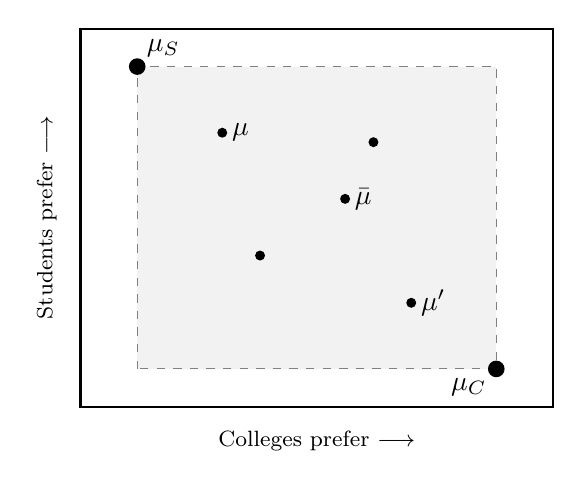
\begin{tikzpicture}[scale=1.2]
    % Box
    \draw[thick] (0,0) rectangle (5,4);
    
    % Axis labels
    \node[below] at (2.5, -0.15) {\footnotesize Colleges prefer $\longrightarrow$};
    \node[rotate=90, anchor=south] at (-0.15, 2) {\footnotesize Students prefer $\longrightarrow$};
    
    % Shaded feasible region
    \fill[gray!10] (0.6, 0.4) rectangle (4.4, 3.6);
    \draw[dashed, gray] (0.6, 0.4) rectangle (4.4, 3.6);
    
    % mu_S: top-left (best for students, worst for colleges)
    \fill (0.6, 3.6) circle (2.5pt) node[above right] {$\mu_S$};
    
    % mu_C: bottom-right (best for colleges, worst for students)
    \fill (4.4, 0.4) circle (2.5pt) node[below left] {$\mu_C$};
    
    % Other stable matchings scattered within the rectangle
    \fill (1.5, 2.9) circle (1.5pt) node[right] {$\mu$};
    \fill (2.8, 2.2) circle (1.5pt) node[right] {$\bar\mu$};
    \fill (3.5, 1.1) circle (1.5pt) node[right] {$\mu'$};
    \fill (1.9, 1.6) circle (1.5pt);
    \fill (3.1, 2.8) circle (1.5pt);
  \end{tikzpicture}
  \end{center}
  Moving toward $\mu_S$ makes every student weakly better off and every college weakly worse off. Moving toward $\mu_C$ does the opposite. Any stable matching must lie weakly within the bounds set by these two extremes.
}

\subsubsection{The Rural Hospital Theorem}

When we allow preferences to include truncations---i.e., agents may find some partners \textit{unacceptable}, so that not every agent is necessarily matched---the following striking result holds.

\thmp{Rural Hospital Theorem (Lone Wolf Theorem)}{
  If a student (or college) is unmatched in \textbf{some} stable matching, then that student (or college) is unmatched in \textbf{all} stable matchings.
}{
  We prove the result for the case of one-to-one matching ($q_c = 1$ for all $c$).
  
  Let $S_u \se \S$ be the set of students unmatched in $\mu_S$ (the student-optimal stable matching), and let $C_u \se \C$ be the set of colleges unmatched in $\mu_S$. Similarly, let $S_u'$ and $C_u'$ be the sets of students and colleges unmatched in $\mu_C$ (the college-optimal stable matching).
  
  \textit{Step 1: $S_u \se S_u'$.} Since $\mu_S$ is the student-optimal stable matching, every student gets their best possible partner across all stable matchings. If a student $s$ is unmatched even in $\mu_S$, then $s$ cannot be matched in any stable matching. In particular, $s$ is unmatched in $\mu_C$. Hence $S_u \se S_u'$.
  
  \textit{Step 2: $C_u' \se C_u$.} By symmetric reasoning, $\mu_C$ is the college-optimal stable matching, so every college gets its best possible partner. If a college $c$ is unmatched in $\mu_C$, then $c$ is unmatched in every stable matching, including $\mu_S$. Hence $C_u' \se C_u$.
  
  \textit{Step 3: Counting argument.} In any one-to-one matching, the number of matched students equals the number of matched colleges. Therefore:
  \[
  |\S| - |S_u| = |\C| - |C_u| \qquad \text{and} \qquad |\S| - |S_u'| = |\C| - |C_u'|.
  \]
  From Step 1, $|S_u| \le |S_u'|$, so the number of matched students in $\mu_S$ is at least the number in $\mu_C$. From Step 2, $|C_u'| \le |C_u|$, so the number of matched colleges in $\mu_C$ is at least the number in $\mu_S$. But matched students $=$ matched colleges in each matching, so:
  \[
  \underbrace{|\S| - |S_u|}_{\text{matched in }\mu_S} \ge \underbrace{|\S| - |S_u'|}_{\text{matched in }\mu_C} = \underbrace{|\C| - |C_u'|}_{\text{matched in }\mu_C} \ge \underbrace{|\C| - |C_u|}_{\text{matched in }\mu_S}.
  \]
  The leftmost and rightmost terms are equal (both count matched pairs in $\mu_S$), so all inequalities are equalities. This forces $|S_u| = |S_u'|$ and $|C_u| = |C_u'|$. Combined with $S_u \se S_u'$ and $C_u' \se C_u$, we conclude:
  \[
  S_u = S_u' \qquad \text{and} \qquad C_u = C_u'.
  \]
  Since every stable matching $\mu$ satisfies $S_u \se S_u^\mu \se S_u'$ (the first inclusion by student-optimality of $\mu_S$, the second by college-optimality of $\mu_C$), and $S_u = S_u'$, we have $S_u^\mu = S_u$ for all stable matchings $\mu$.
}

\rmkb{
  The name ``Rural Hospital'' comes from the practical observation in medical residency matching: hospitals in rural areas that fail to fill all their positions under one stable matching will fail to fill them under \textit{every} stable matching. Switching from the hospital-proposing to the resident-proposing DA (or any other stable mechanism) cannot help a rural hospital that is fundamentally undesirable to residents. The set of matched agents is invariant across stable matchings---only the \textit{partners} can change, not whether one is matched at all.
}

\section{The Boston Mechanism (Immediate Acceptance)}

To truly appreciate the elegance and power of the Deferred Acceptance (DA) algorithm, it is instructive to study a mechanism that attempts to solve the same problem but fails spectacularly in its theoretical properties. The most famous example is the \textbf{Boston Mechanism}, historically used by the Boston Public School system (and many other school districts worldwide) before economists pointed out its severe flaws.

The Boston Mechanism is also known as the \textbf{Immediate Acceptance} mechanism. The critical difference from DA lies in the word ``immediate'': once a college accepts a student, that decision is permanent. Seats are locked in, and future applicants cannot displace already-admitted students, regardless of how highly the college ranks the new applicants.

\defn{The Boston Mechanism}{
  \begin{enumerate}
    \item \textbf{Round 1:} Each student proposes to their first-choice college. Each college looks at its proposals, accepts its most preferred students up to its quota, and rejects the rest. \textbf{These acceptances are final.} The college's quota is reduced accordingly.
    \item \textbf{Round $k$ ($k \ge 2$):} Each student rejected in Round $k-1$ proposes to their $k$-th choice college. Each college looks at its \textit{remaining} unfilled seats (if any). It accepts its most preferred students among the new applicants up to its remaining quota, and rejects the rest. \textbf{These acceptances are final.}
    \item \textbf{Repeat} until all students are matched or all available seats are filled.
  \end{enumerate}
}

\ex[Boston Mechanism on the 10x10 Matching Problem]{
  Let us apply the Boston Mechanism to the exact same 10-student, 10-college problem. All colleges have quota $q = 1$. 

\medskip
\noindent\textbf{College preferences (Boston Mechanism final matches highlighted):}
\begin{center}
\renewcommand{\arraystretch}{1.15} 
\small 
\begin{tabular}{c|cccccccccc}
    Rank & $c_1$ & $c_2$ & $c_3$ & $c_4$ & $c_5$ & $c_6$ & $c_7$ & $c_8$ & $c_9$ & $c_{10}$ \\
    \hline
    1 & $s_1$ & $s_1$ & $s_{10}$ & $s_6$ & $s_7$ & $s_4$ & $s_1$ & $s_6$ & $s_8$ & $s_6$ \\
    2 & $s_2$ & $s_6$ & $s_2$ & $s_1$ & $s_2$ & $s_8$ & $s_4$ & $s_4$ & $s_{10}$ & $s_5$ \\
    3 & $s_3$ & $s_9$ & $s_4$ & $s_5$ & $s_8$ & $s_2$ & $s_3$ & $s_2$ & $s_6$ & \match{s_1} \\
    4 & $s_4$ & $s_2$ & \match{s_6} & \match{s_2} & $s_4$ & $s_6$ & $s_8$ & $s_{10}$ & \match{s_9} & $s_4$ \\
    5 & $s_5$ & $s_5$ & $s_8$ & $s_7$ & $s_{10}$ & $s_{10}$ & \match{s_5} & $s_8$ & $s_5$ & $s_{10}$ \\
    6 & $s_6$ & $s_8$ & $s_3$ & $s_3$ & $s_5$ & $s_3$ & $s_2$ & $s_3$ & $s_7$ & $s_8$ \\
    7 & $s_7$ & $s_3$ & $s_5$ & $s_8$ & $s_9$ & $s_7$ & $s_9$ & $s_1$ & $s_4$ & $s_9$ \\
    8 & \match{s_8} & $s_4$ & $s_7$ & $s_4$ & $s_6$ & $s_1$ & $s_6$ & $s_9$ & $s_3$ & $s_2$ \\
    9 & $s_9$ & $s_7$ & $s_9$ & $s_{10}$ & \match{s_3} & $s_5$ & $s_7$ & \match{s_7} & $s_1$ & $s_3$ \\
    10 & $s_{10}$ & \match{s_{10}} & $s_1$ & $s_9$ & $s_1$ & $s_9$ & $s_{10}$ & $s_5$ & $s_2$ & $s_7$ \\
\end{tabular}
\end{center}

\medskip
\noindent\textbf{Student preferences (Boston Mechanism final matches highlighted):}
\begin{center}
\renewcommand{\arraystretch}{1.15}
\small
\begin{tabular}{c|cccccccccc}
    Rank & $s_1$ & $s_2$ & $s_3$ & $s_4$ & $s_5$ & $s_6$ & $s_7$ & $s_8$ & $s_9$ & $s_{10}$ \\
    \hline
    1 & $c_5$ & \match{c_4} & \match{c_5} & \match{c_6} & $c_3$ & \match{c_3} & \match{c_8} & \match{c_1} & $c_1$ & \match{c_2} \\
    2 & \match{c_{10}} & $c_9$ & $c_6$ & $c_2$ & \match{c_7} & $c_4$ & $c_6$ & $c_4$ & $c_5$ & $c_{10}$ \\
    3 & $c_6$ & $c_{10}$ & $c_1$ & $c_5$ & $c_9$ & $c_5$ & $c_4$ & $c_2$ & $c_2$ & $c_9$ \\
    4 & $c_4$ & $c_6$ & $c_7$ & $c_8$ & $c_{10}$ & $c_1$ & $c_2$ & $c_6$ & $c_{10}$ & $c_4$ \\
    5 & $c_7$ & $c_3$ & $c_4$ & $c_1$ & $c_1$ & $c_9$ & $c_9$ & $c_3$ & $c_3$ & $c_1$ \\
    6 & $c_2$ & $c_7$ & $c_8$ & $c_7$ & $c_5$ & $c_7$ & $c_7$ & $c_7$ & $c_8$ & $c_7$ \\
    7 & $c_8$ & $c_1$ & $c_9$ & $c_3$ & $c_4$ & $c_{10}$ & $c_5$ & $c_5$ & $c_6$ & $c_5$ \\
    8 & $c_9$ & $c_5$ & $c_{10}$ & $c_9$ & $c_2$ & $c_8$ & $c_{10}$ & $c_{10}$ & $c_7$ & $c_6$ \\
    9 & $c_1$ & $c_2$ & $c_2$ & $c_{10}$ & $c_6$ & $c_2$ & $c_1$ & $c_8$ & $c_4$ & $c_3$ \\
    10 & $c_3$ & $c_8$ & $c_3$ & $c_4$ & $c_8$ & $c_6$ & $c_3$ & $c_9$ & \match{c_9} & $c_8$ \\
\end{tabular}
\end{center}

\vspace{0.3cm}
We use the same chalkboard-style simulation. However, green text now represents a \textbf{permanent acceptance} (\textcolor{ForestGreen}{\textbf{admitted}}), rather than a tentative hold. Once a column is filled with a green student, that college is closed forever.

\medskip
\noindent\textbf{Round 1.} \\
All 10 students propose to their first-choice colleges.
\begin{center}
\renewcommand{\arraystretch}{1.2}
\begin{tabular}{cccccccccc}
    $c_1$ & $c_2$ & $c_3$ & $c_4$ & $c_5$ & $c_6$ & $c_7$ & $c_8$ & $c_9$ & $c_{10}$ \\
    \hline
    \textcolor{ForestGreen}{$\mathbf{s_8}$} & \textcolor{ForestGreen}{$\mathbf{s_{10}}$} & \textcolor{ForestGreen}{$\mathbf{s_6}$} & \textcolor{ForestGreen}{$\mathbf{s_2}$} & \textcolor{ForestGreen}{$\mathbf{s_3}$} & \textcolor{ForestGreen}{$\mathbf{s_4}$} & & \textcolor{ForestGreen}{$\mathbf{s_7}$} & & \\
    $\cancel{s_9}$ & & $\cancel{s_5}$ & & $\cancel{s_1}$ & & & & & \\
\end{tabular}
\end{center}
\textit{Explanation:} Colleges $c_2, c_4, c_6, c_8$ receive exactly one applicant and admit them immediately. Colleges $c_1, c_3, c_5$ face competition. They admit their preferred applicant ($s_8, s_6, s_3$ respectively) and reject the rest. \\
\textit{Status:} Colleges $c_1, c_2, c_3, c_4, c_5, c_6, c_8$ are now \textbf{permanently closed}. \\
\textit{Rejected:} $s_9$ (next $c_5$), $s_5$ (next $c_7$), $s_1$ (next $c_{10}$).

\medskip
\noindent\textbf{Round 2.} \\
The three rejected students propose to their second-choice colleges. 
\begin{center}
\renewcommand{\arraystretch}{1.2}
\begin{tabular}{cccccccccc}
    \cellcolor{gray!20}$c_1$ & \cellcolor{gray!20}$c_2$ & \cellcolor{gray!20}$c_3$ & \cellcolor{gray!20}$c_4$ & \cellcolor{gray!20}$c_5$ & \cellcolor{gray!20}$c_6$ & $c_7$ & \cellcolor{gray!20}$c_8$ & $c_9$ & $c_{10}$ \\
    \hline
    & & & & \textbf{FULL} & & \textcolor{ForestGreen}{$\mathbf{s_5}$} & & & \textcolor{ForestGreen}{$\mathbf{s_1}$} \\
    & & & & $\cancel{s_9}$ & & & & & \\
\end{tabular}
\end{center}
\textit{Explanation:} Students $s_1$ and $s_5$ apply to $c_{10}$ and $c_7$, which are still empty. They are admitted permanently. Student $s_9$ applies to $c_5$. However, $c_5$ was already filled by $s_3$ in Round 1! Even though $c_5$ prefers $s_9$ (\#7) over $s_3$ (\#9), it is too late. The seat is gone. $s_9$ is automatically rejected. \\
\textit{Status:} Colleges $c_7, c_{10}$ are now \textbf{permanently closed}. Only $c_9$ remains open. \\
\textit{Rejected:} $s_9$ (next $c_2$).

\medskip
\noindent\textbf{Rounds 3 through 9 (The Free-Fall of $s_9$).} \\
Student $s_9$ has suffered a ``cascading failure'' (滑档). Because he missed his first choice, he is now applying to colleges that were filled in Round 1. 
\begin{itemize}
    \item \textbf{Round 3:} $s_9 \to c_2$. \textbf{FULL} (filled by $s_{10}$). Rejected.
    \item \textbf{Round 4:} $s_9 \to c_{10}$. \textbf{FULL} (filled by $s_1$). Rejected.
    \item \textbf{Round 5:} $s_9 \to c_3$. \textbf{FULL} (filled by $s_6$). Rejected.
    \item \textbf{Round 6:} $s_9 \to c_8$. \textbf{FULL} (filled by $s_7$). Rejected.
    \item \textbf{Round 7:} $s_9 \to c_6$. \textbf{FULL} (filled by $s_4$). Rejected.
    \item \textbf{Round 8:} $s_9 \to c_7$. \textbf{FULL} (filled by $s_5$). Rejected.
    \item \textbf{Round 9:} $s_9 \to c_4$. \textbf{FULL} (filled by $s_2$). Rejected.
\end{itemize}

\medskip
\noindent\textbf{Round 10.} \\
Student $s_9$ finally reaches his 10th and absolute worst choice, $c_9$. Luckily, $c_9$ is still empty.
\begin{center}
\renewcommand{\arraystretch}{1.2}
\begin{tabular}{cccccccccc}
    \cellcolor{gray!20}$c_1$ & \cellcolor{gray!20}$c_2$ & \cellcolor{gray!20}$c_3$ & \cellcolor{gray!20}$c_4$ & \cellcolor{gray!20}$c_5$ & \cellcolor{gray!20}$c_6$ & \cellcolor{gray!20}$c_7$ & \cellcolor{gray!20}$c_8$ & $c_9$ & \cellcolor{gray!20}$c_{10}$ \\
    \hline
     & & & & & & & & \textcolor{ForestGreen}{$\mathbf{s_9}$} & \\
\end{tabular}
\end{center}
\textit{The algorithm terminates.}

\vspace{0.5cm}
\noindent The \textbf{Boston Mechanism matching} $\mu_B$ is:
\[
\begin{array}{c|cccccccccc}
  \text{College} & c_1 & c_2 & c_3 & c_4 & c_5 & c_6
                 & c_7 & c_8 & c_9 & c_{10} \\
  \hline
  \text{Student} & s_8 & s_{10} & s_6 & s_2 & s_3
                 & s_4 & s_5 & s_7 & s_9 & s_1
\end{array}
\]
}

\subsection{Properties of the Boston Mechanism}

The simulation above provides everything we need to expose the theoretical failures of the Boston Mechanism. We examine the two most important properties: Pairwise Stability and Strategy-Proofness.

\thmp{The Boston Mechanism is NOT Stable}{
  The allocation produced by the Boston Mechanism may contain blocking pairs, meaning it fails to guarantee a pairwise stable matching.
}{
  We can prove this by simply identifying a blocking pair in the outcome $\mu_B$ of our example. 
  
  Under $\mu_B$, student $s_9$ is matched with $c_9$ (his 10th choice), and college $c_5$ is matched with $s_3$ (its 9th choice). 
  Now look at their true preferences:
  \begin{itemize}
      \item Student $s_9$ ranks $c_5$ as his 2nd choice, meaning $c_5 \succ_{s_9} \mu_B(s_9) = c_9$.
      \item College $c_5$ ranks $s_9$ as its 7th choice, meaning $s_9 \succ_{c_5} \mu_B(c_5) = s_3$.
  \end{itemize}
  Both $s_9$ and $c_5$ would strictly prefer to be matched with each other rather than their current assignments. Thus, \textbf{$(c_5, s_9)$ forms a blocking pair}. 
  
  The instability arises precisely because of the ``immediate acceptance'' rule: $c_5$ was forced to permanently commit to $s_3$ in Round 1, preventing it from accepting the much stronger applicant $s_9$ who arrived in Round 2.
}

\thmp{The Boston Mechanism is NOT Strategy-Proof}{
  Under the Boston Mechanism, truthful reporting is not a dominant strategy. Students can often obtain a strictly better outcome by misreporting their preferences.
}{
  \rmk{
    Because missing out on your first choice is heavily penalized (the ``free-fall'' effect seen with $s_9$), the Boston Mechanism forces students to play a high-stakes psychological game. Instead of ranking their true favorite first, students are incentivized to rank a ``safe'' school first to secure a seat in Round 1.
  }

  We demonstrate this with student $s_9$ from our example. Under truthful reporting, $s_9$ listed $c_1$ as his 1st choice and $c_5$ as his 2nd choice. Because he lost the tie-breaker at $c_1$ in Round 1, he free-fell all the way to $c_9$, his worst possible outcome.

  \medskip
  Suppose $s_9$ anticipates this and decides to deviate. He submits a fake preference list $P_{s_9}'$ where he promotes his 2nd choice ($c_5$) to his 1st choice, abandoning the highly competitive $c_1$. The rest of the students report truthfully.

\medskip
\noindent\textbf{Modified Student Preferences (with $s_9$'s misreport highlighted in blue):}
\begin{center}
\renewcommand{\arraystretch}{1.15}
\small
\begin{tabular}{c|cccccccc>{\columncolor{blue!10}}cc}
    Rank & $s_1$ & $s_2$ & $s_3$ & $s_4$ & $s_5$ & $s_6$ & $s_7$ & $s_8$ & $\mathbf{s_9'}$ & $s_{10}$ \\
    \hline
    1 & $c_5$ & $c_4$ & $c_5$ & $c_6$ & $c_3$ & $c_3$ & $c_8$ & $c_1$ & \textcolor{blue}{$\mathbf{c_5}$} & $c_2$ \\
    2 & $c_{10}$ & $c_9$ & $c_6$ & $c_2$ & $c_7$ & $c_4$ & $c_6$ & $c_4$ & \textcolor{blue}{$\mathbf{c_1}$} & $c_{10}$ \\
    3 & $c_6$ & $c_{10}$ & $c_1$ & $c_5$ & $c_9$ & $c_5$ & $c_4$ & $c_2$ & $c_2$ & $c_9$ \\
    4 & $c_4$ & $c_6$ & $c_7$ & $c_8$ & $c_{10}$ & $c_1$ & $c_2$ & $c_6$ & $c_{10}$ & $c_4$ \\
    $\vdots$ & $\vdots$ & $\vdots$ & $\vdots$ & $\vdots$ & $\vdots$ & $\vdots$ & $\vdots$ & $\vdots$ & $\vdots$ & $\vdots$ \\
\end{tabular}
\end{center}

  Let us trace \textbf{Round 1} of the Boston Mechanism under this new profile. All students apply to their reported 1st choices. 
  
\begin{center}
\renewcommand{\arraystretch}{1.2}
\begin{tabular}{cccccccccc}
    $c_1$ & $c_2$ & $c_3$ & $c_4$ & $c_5$ & $c_6$ & $c_7$ & $c_8$ & $c_9$ & $c_{10}$ \\
    \hline
    \textcolor{ForestGreen}{$\mathbf{s_8}$} & \textcolor{ForestGreen}{$\mathbf{s_{10}}$} & \textcolor{ForestGreen}{$\mathbf{s_6}$} & \textcolor{ForestGreen}{$\mathbf{s_2}$} & \textcolor{ForestGreen}{$\mathbf{s_9}$} & \textcolor{ForestGreen}{$\mathbf{s_4}$} & & \textcolor{ForestGreen}{$\mathbf{s_7}$} & & \\
     & & $\cancel{s_5}$ & & $\cancel{s_3}$ & & & & & \\
     & & & & $\cancel{s_1}$ & & & & & \\
\end{tabular}
\end{center}
  
  \textit{Explanation of $c_5$'s decision:} 
  College $c_5$ now receives Round 1 proposals from $s_1$, $s_3$, and the strategically misreporting $s_9$. 
  Looking at $c_5$'s true preference list: $s_9$ (\#7) $\succ_{c_5} s_3$ (\#9) $\succ_{c_5} s_1$ (\#10). 
  Because $c_5$ evaluates all three applicants simultaneously in Round 1, it permanently admits its favorite among them: \textbf{$s_9$}.

  \medskip
  \noindent By lying and placing $c_5$ first, student $s_9$ completely avoided the free-fall and secured his true 2nd choice ($c_5$). This outcome is strictly better for him than the 10th choice ($c_9$) he received when telling the truth. Since a profitable deviation exists, the Boston mechanism is \textbf{not strategy-proof}.
}

\rmkb[The Tragedy of the Boston Mechanism]{
  The Boston Mechanism systematically rewards sophisticated, strategic families while punishing honest, naive ones. A naive student who truthfully applies to a competitive "reach" school wastes their critical Round 1 proposal. By the time they are rejected and move to their "match" schools in Round 2, those schools have already been filled by strategic students who ranked them first. This profound inequity is why many school districts have replaced it with the Strategy-Proof Deferred Acceptance algorithm.
}

